\documentclass[11pt]{article}
\usepackage{enumitem}
\usepackage{hyperref}
\hypersetup{
	colorlinks=true,
	linkcolor=blue,
	filecolor=magenta,      
	urlcolor=cyan,
}
\usepackage{graphicx}
\usepackage{amsmath}
\usepackage[utf8]{inputenc}
\usepackage{mathtools}
\usepackage[caption=false]{subfig}
\usepackage{soul}
\usepackage[top=0.75in, bottom=0.75in, left=1in, right=1in]{geometry}
\usepackage[margin=1.5cm]{caption}
\usepackage{epsfig,amsmath}
\DeclarePairedDelimiter\abs{${\lvert}$}{${\rvert}$}%
\usepackage{titlesec,color}
\usepackage{kpfonts}
\usepackage{empheq}
\usepackage{palatino}
\usepackage{graphicx,wrapfig}
\setlength{\parskip}{1em}
\setlength{\parindent}{0pt}
\usepackage{array}
\usepackage{gensymb}
\usepackage{soul}
\usepackage{grffile}
\usepackage{multicol}
\usepackage{listings}
\usepackage{color}
\usepackage{tcolorbox}
\usepackage{courier}
\usepackage[T1]{fontenc}
\tcbuselibrary{listings,skins}

\lstdefinestyle{mystyle}{
	basicstyle=\small\ttfamily,
	numbers=none,
	language=MATLAB
}


\newtcblisting{mylisting}[2][]{
	arc=0pt, outer arc=0pt,
	listing only, 
	listing style=mystyle,
	title=#2,
	#1
}



\definecolor{dkgreen}{rgb}{0,0.6,0}
\definecolor{gray}{rgb}{0.5,0.5,0.5}
\definecolor{mauve}{rgb}{0.58,0,0.82}

\lstset{frame=tb,
	language=MATLAB,
	aboveskip=3mm,
	belowskip=3mm,
	showstringspaces=false,
	columns=flexible,
	basicstyle={\small\ttfamily},
	numbers=none,
	numberstyle=\tiny\color{gray},
	keywordstyle=\color{blue},
	commentstyle=\color{dkgreen},
	stringstyle=\color{mauve},
	breaklines=true,
	breakatwhitespace=true,
	tabsize=3
}


\begin{document}
	
\renewcommand*\rmdefault{phv}
\fontfamily{phv}\selectfont
	
\title{MARGO - User Manual}
\maketitle

\newcommand{\avg}[1]{\left<{#1}\right>}
\newcommand{\hence}{\hspace{1cm}\Longrightarrow\hspace{1cm}}
\renewcommand{\ni}{\noindent}
\newcommand{\din}{\indent \indent}
\newcommand{\mni}{\medskip \noindent}
\newcommand{\bni}{\bigskip \noindent}
\newcommand{\sni}{\smallskip \noindent}
\newcommand{\pr}{{\rm Prob}}
\newcommand{\mon}{\begin{displaymath}}
\newcommand{\moff}{\end{displaymath}}
\newcommand{\sumi}[1]{\sum_{{#1}=-\infty}^{\infty}}
\renewcommand{\b}[1]{\mbox{\boldmath ${#1}$}}
\newcommand{\sumy}{\sum_{\b{y}}}
\newcommand{\sumz}{\sum_{\b{z}}}
\newcommand{\pd}[2]{\frac{\partial {#1}}{\partial {#2}}}
\newcommand{\od}[2]{\frac{d {#1}}{d {#2}}}
\newcommand{\odat}[3]{\left. \frac{d {#1}}{d {#2}} \right|_{#3}}
\newcommand{\inti}{\int_{-\infty}^{\infty}}
\newcommand{\eon}{\begin{equation}}
\newcommand{\eoff}{\end{equation}}
\newcommand{\eaon}{\begin{eqnarray}}
\newcommand{\eaoff}{\end{eqnarray}}
\newcommand{\e}[1]{\times 10^{#1}}
\newcommand{\chem}[2]{{}^{#2} \mathrm{#1}}
\renewcommand{\sb}{s}
\newcommand{\s}{s}
\newcommand{\zetaexp}{\left( \zeta e^{q \s t} \right)}
\newcommand{\taunuc}{\tau_{nuc}}
\newcommand{\eq}[1]{Eq. (\ref{#1})}\
\newcommand{\ev}[1]{\langle #1 \rangle}
\newcommand*\mean[1]{${\bar{#1}}$}
\newcolumntype{L}{>{\centering\arraybackslash}m{5cm}}

\cleardoublepage


\tableofcontents

\newpage
\section{Introduction}

\subsection{Quickstart Guide}

\begin{figure}[h!]
	\begin{center}
		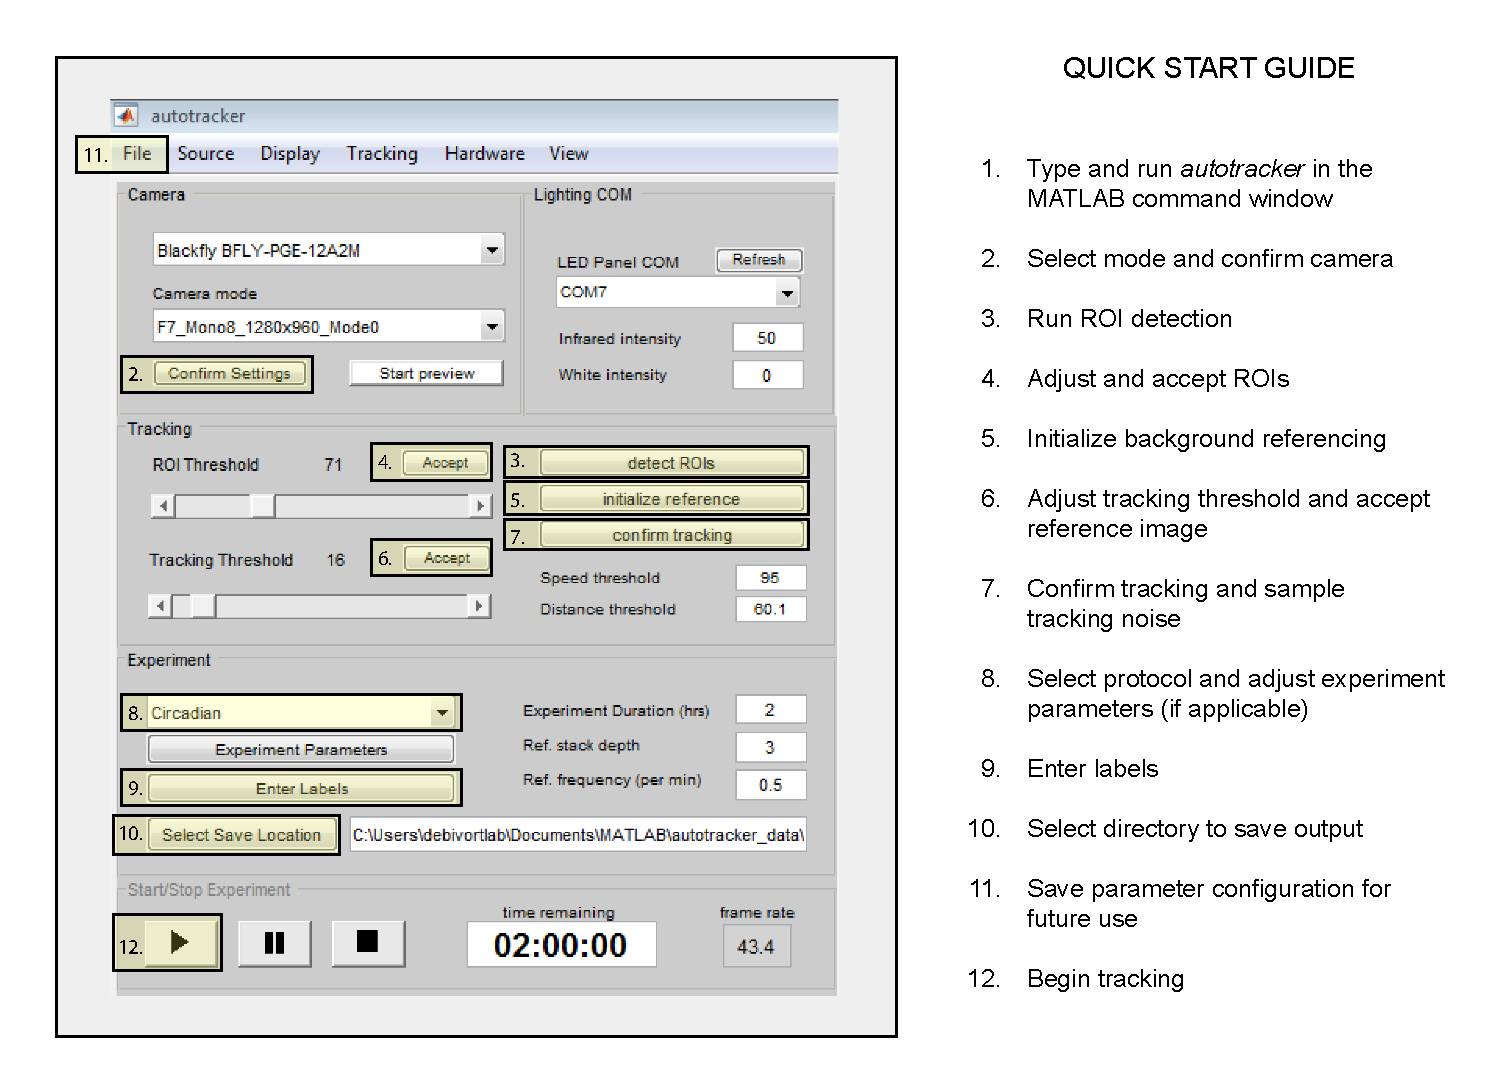
\includegraphics[width=0.95\textwidth]{images/quickstart/quick_start_guide.pdf}
	\end{center}
\end{figure}

\begin{figure}[h!]
	\begin{center}
		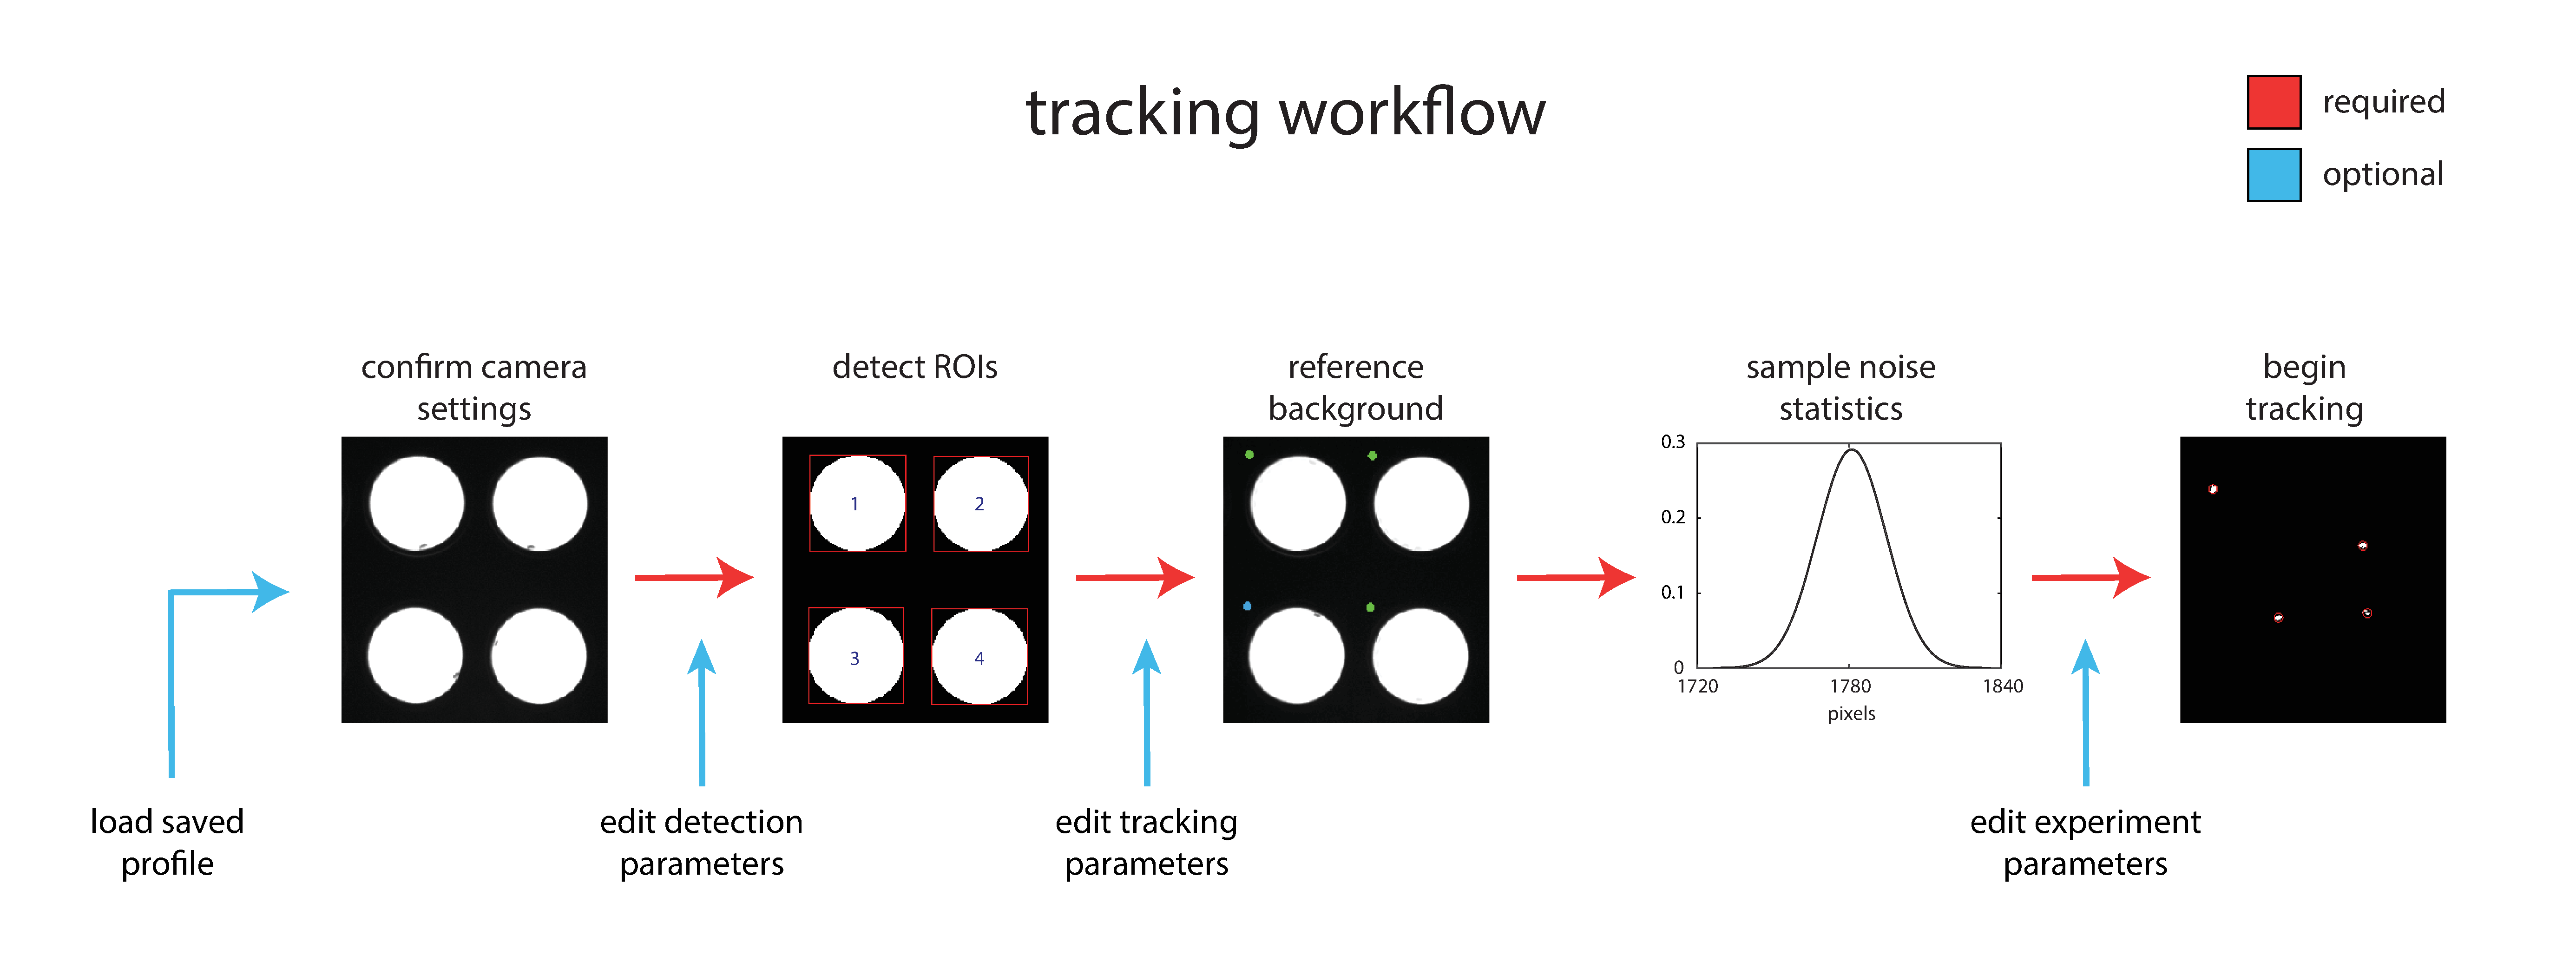
\includegraphics[width=0.95\textwidth]{images/getting_started/tracking_workflow.pdf}
	\end{center}
	\caption*{\footnotesize {\textit{figure 1.1} - Every tracking session follows a standard workflow with multiple stages for optional customization. The time needed to setup a new session can be substantially reduced by loading saved parameters.}}
\end{figure}

\subsection{Overview}

MARGO is a MATLAB-based software package for real-time, high-throughput tracking of animals. Rapid tracking and identity sorting in real-time means that MARGO is particularly useful for applications requiring closed-loop control of individual stimulus delivery and massively high-throughput behavioral screens where video storage and processing would otherwise be rate-limiting. Margo has two fundamental modes of tracking: 
\begin{enumerate}
	\item \textbf{Single Trackin}g - This mode is designed to track spatially segregated animals in parallel. Spatial segregation allows individuals to be tracked separately in defined regions of interest (ROIs). Single tracking operates on a single animal per ROI and can track many hundreds or thousands of individuals in parallel at high acquisition rates. In this mode, individual identities can be maintained indefinitely without supervision.
	\item \textbf{Multi Tracking} - This mode is designed to track groups of animals in parallel in one or more ROIs. Multi tracking can be used to track spatial distribution, activity level, and group dynamics that do not require maintenance of individual identities.
\end{enumerate}
Many existing tracking platforms such as Ctrax, idTracker, and FlyTracker are designed to track and maintain individual identities of mixed groups individuals. Tracking identity in mixed groups requires resolving identities through collisions where bodies are overlapping. This approach offers the ability to study social behaviors, but because collision resolution is computationally expensive, software packages focused on solving this perform acquisition and tracking separately. Assigning centroid identity by associating individual with a predefined region of interest (ROI) allows MARGO to track individuals in real-time and avoid recording image data altogether. 

MARGO offers additional utility through extensive GUI-based customization of hardware settings, advanced tracking parameters, ROI-detection modes, and saved preferences. In addition to centroid data, MARGO can output timestamps, body orientation, body size, speed, heading direction, angular velocity, and other custom defined metrics. Support for cameras, external displays, and serial COM devices make it possible to integrate hardware into experimental paradigms. MARGO facilitates experimental paradigms that require closed loop control of individual stimuli based on individual behavior. Furthermore, a small data footprint and robustness to tracking noise makes MARGO ideal for recording behavior over long time scales.

\subsection{Target audience}

The target audience of MARGO is any user wanting to use a single, integrated platform for recording body position and orientation based behavioral metrics over time, particularly for applications requiring any of the following: 1) tracking hundreds to thousands of individuals simultaneously with little to no human intervention 2) closed-loop feedback between real-time tracking data and control of hardware. Many features of behavior can be calculated or inferred from these simple pieces of information. To extract these measurements, MARGO uses thresholded images to track binary blobs. This means that the software is optimized for tracking many individuals at very low-resolution and not for high-resolution tracking of postural subfeatures (eg. tracking positions or orientations of individual body parts). Relying in ROIs to track individual identity also means that MARGO is built for high-throughput experiments where individuals are physically separated into isolated arenas (eg. bottomless 96 well plates). MARGO is not designed for collision resolution and therefore does not track the identities of multiple individuals sharing the same arena. 

\newpage
\subsection{Experimental workflow}

Every live experiment conducted in MARGO follows the same fundamental workflow to ensure that the software assign regions of interest, separates the interesting parts of the image from background, and filters out noise in the image that would otherwise cause errors in centroid estimation. Before recording data, the user must:

\begin{enumerate}
	\itemsep0em 
	\item Select and confirm settings for the camera
	\item Automatically or manually set ROIs
	\item Initialize a background reference image
	\item Collect a sample of clean imaging
	\item Set experiment parameters
\end{enumerate}

\begin{figure}[h!]
	\begin{center}
		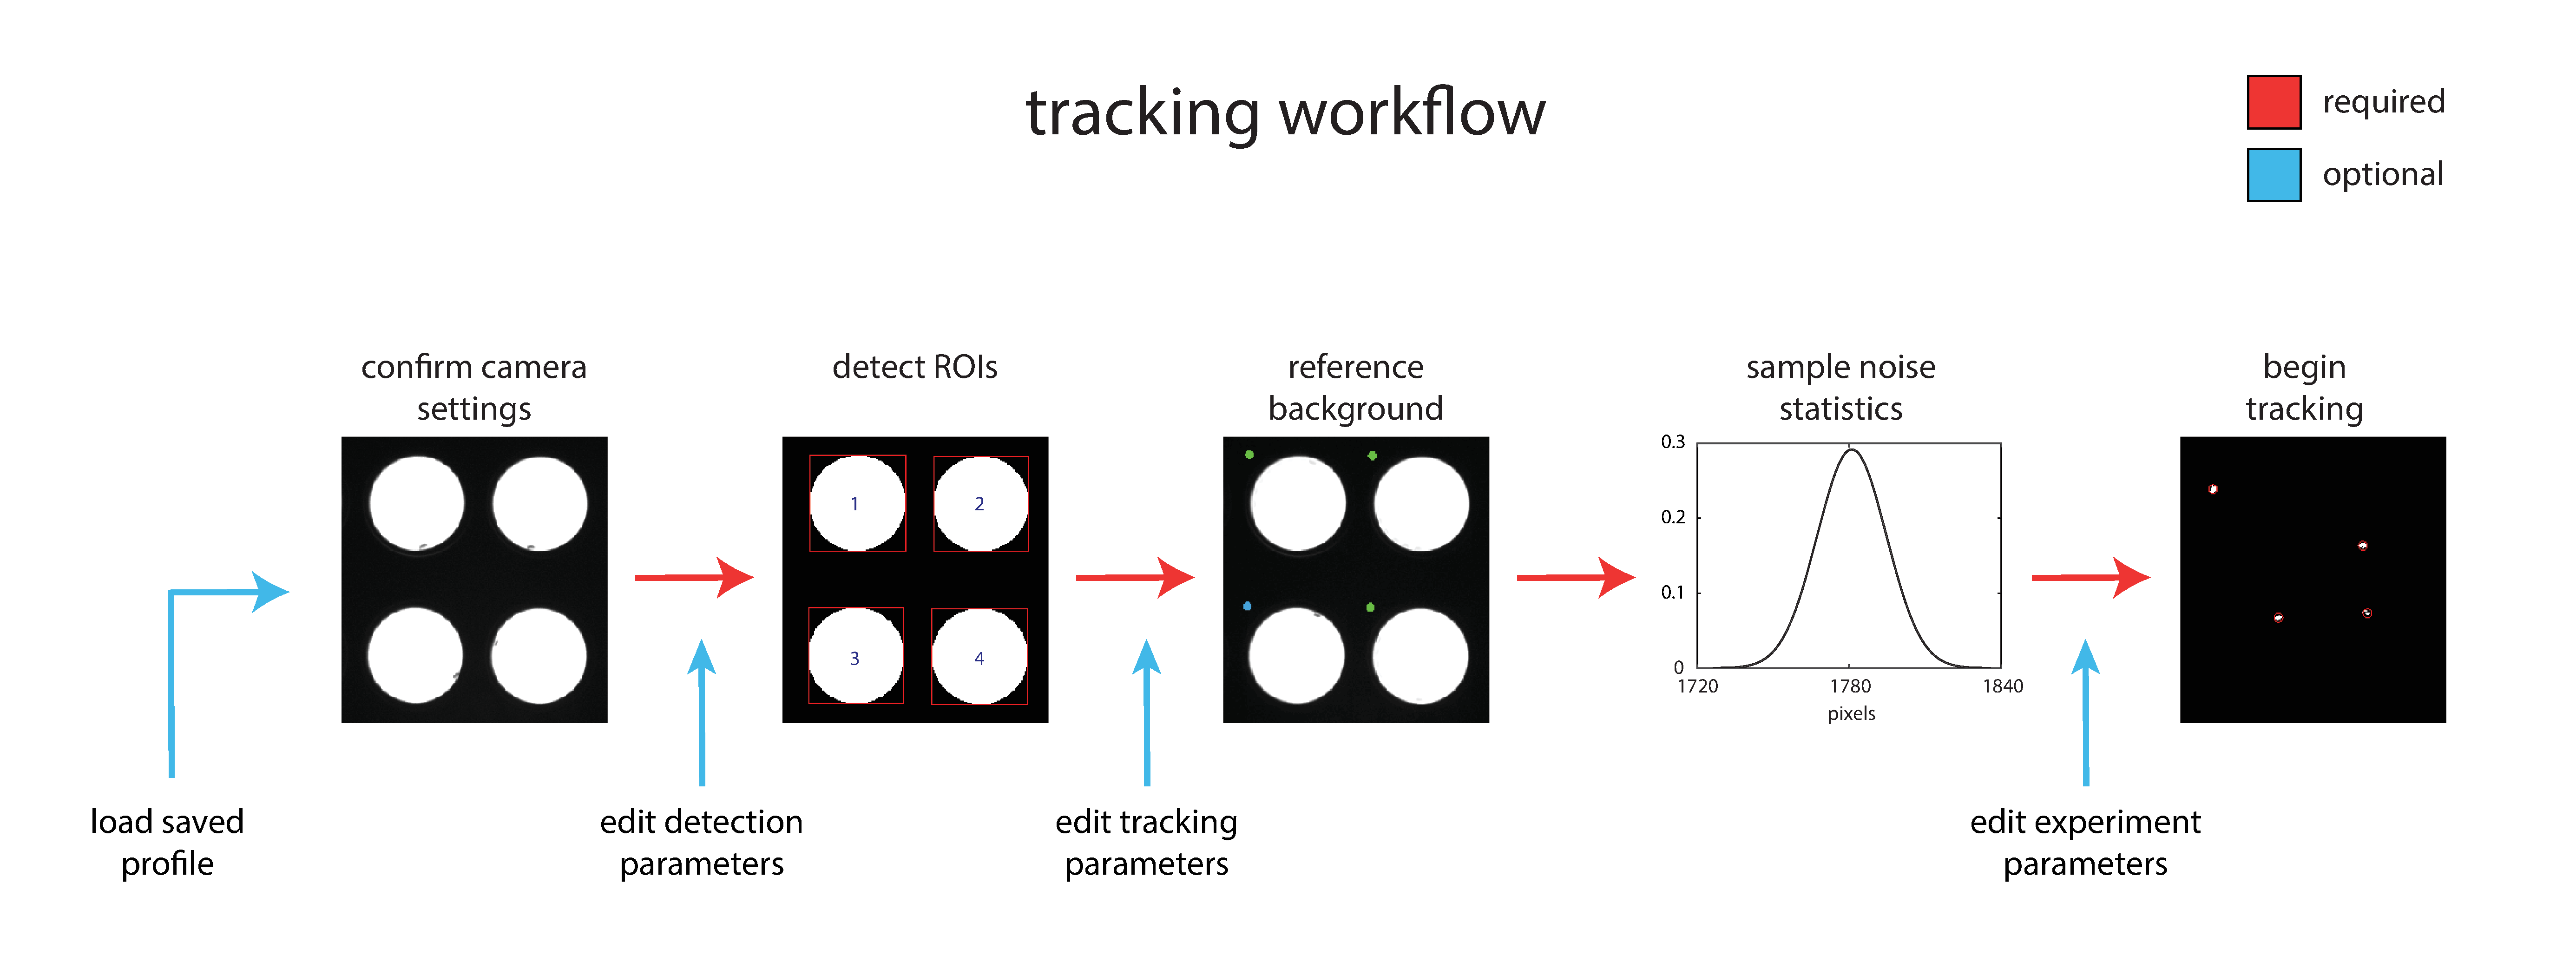
\includegraphics[width=0.95\textwidth]{images/getting_started/tracking_workflow.pdf}
	\end{center}
	\caption*{\footnotesize {\textit{figure 1.3} - Every tracking session follows a standard workflow with multiple stages for optional customization. The time needed to setup a new session can be substantially reduced by loading saved parameters.}}
\end{figure}

\fontsize{10}{0}
\textbf{Select and confirm settings for the camera}

MARGO will automatically detect any available camera with an associated MATLAB imaq adaptor installed and auto-populate the camera panel drop down with detected cameras. If no cameras are detected, see \hyperlink{camdetect}{Camera detection} for information on installing MATLAB camera adaptors. Select the appropriate camera and the camera mode and click "Confirm Settings". After initializing the camera, an initial preview image will be visible in the display window and the downstream ROI detection controls will be enabled. The camera preview button can be used to start and stop a streaming preview from the camera at any time the camera is not actively in use.

\begin{figure}[h!]
	%\vspace*{0.75cm}
	\begin{center}
		%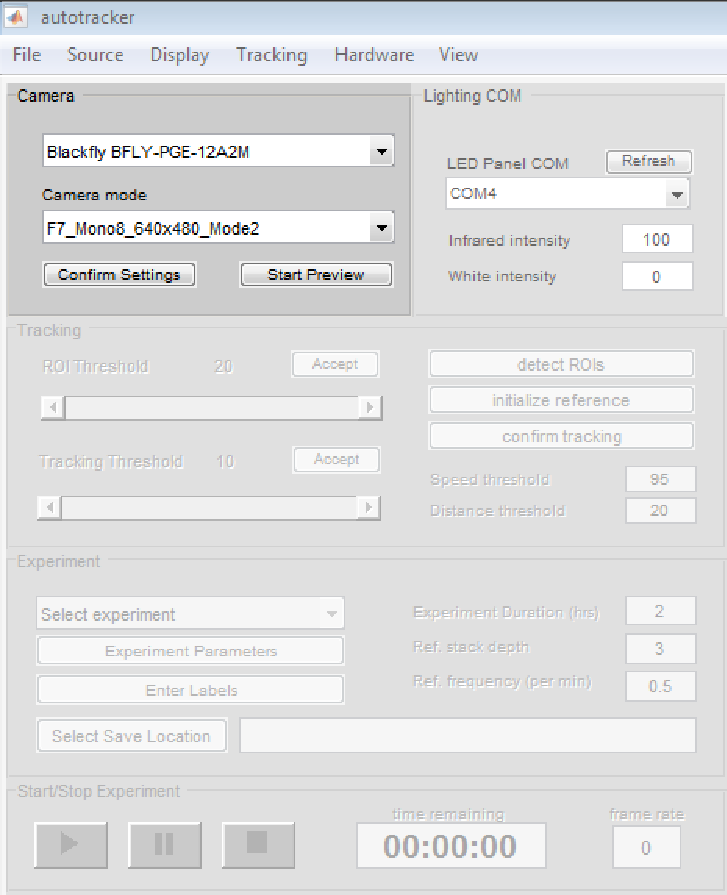
\includegraphics[width=0.5\textwidth]{images/getting_started/MARGO_gui/startup_filt.pdf}
	\end{center}
	\footnotesize {}
\end{figure}

\fontsize{10}{0}
\textbf{Automatically or manually select ROIs} 

Before individual identities can be tracked frame to frame, regions of interest must be set. MARGO sets ROIs through either \textit{automatic} or \textit{grid} modes. ROI detection mode is set to automatic by default. Automatic ROI detection works on two fundamental assumptions. The first is that your ROIs will be bright regions separated by dark boundaries. The second is that ROIs will all generally be about the same size. To run automatic ROI detection, select \textbf{\textit{detect ROIs}} and adjust the ROI threshold slider bar to find a threshold that cleanly separates ROIs from the background. Bounding boxes and ROI numbers will be displayed over any detected ROIs in real time. Select \textbf{\textit{Accept}} once the ROIs are properly detected to confirm the ROI positions. See \hyperlink{roidetect}{ROI detection} for more information on automatic and grid based ROI detection modes.


\fontsize{10}{0}
\textbf{Initialize a background reference image}

To track changes in the image from frame to frame, MARGO calculates a difference image between each frame and a background reference image. The background reference is generated by computing a median image from snapshots of each ROI when the individual is in different locations. This effectively generates an image of the ROIs without individuals. In order for this strategy to work, MARGO must be able to track individuals in each ROI to ensure that the individual is in distinct locations each time a new image is taken. To collect a reference image, select "initialize reference" and adjust the tracking threshold slider until individuals are detected. Colored indicators next to each ROI will progress from purple to green as sample images of each ROI are collected. The "centroid numbers" option in the View menu bar can be selected at any time to visualize the assignment of centroid identity. See \hyperlink{initializeref}{Background referencing} for more information on how to optimize a starting reference image.

\subsection{Getting the most out of MARGO}

Fast, accurate tracking can be highly dependent on optimization of parameters, camera configuration, and illumination. MARGO attempts to make the task from setup to data collection as streamlined as possible by making some of these decisions for you. Since every experiment and tracking setup is a bit different, getting optimal tracking performance out of MARGO may require adjusting both software and hardware parameters. MARGO has many integrated features to help the user make these decisions and then save the preferences to a user profile to ensure that the setup process is only necessary once. Here is a helpful but non-comprehensive list of things that will help you get the most out of MARGO: 

\vspace*{0.15cm}
\small
\underline{high priority}
\vspace*{-0.45cm}
\begin{itemize}
	\itemsep0em 
	\item \hyperlink{arenasection}{Behavioral arenas that facilitate ROI detection} 
	\item \hyperlink{illumsection}{Bright, diffuse backlighting}
	\item \hyperlink{camconfig}{Proper camera configuration}
	\item \hyperlink{trackingparam}{Tracking parameters customized to your ROIs and tracked objects}
	\item \hyperlink{targetrate}{Adjust acquisition rate to avoid "over-tracking"}
	\item \hyperlink{saveprofile}{Save your settings to a profile}
\end{itemize}
\vspace*{-0.15cm}
\underline{recommended}
\vspace*{-0.45cm}
\begin{itemize}
	\itemsep0em 
	\item \hyperlink{camcalibrate}{Camera calibration to reduce lens fisheye} 
	\item \hyperlink{viewoptions}{Use display options to visualize and validate tracking features in real time}
	\item \hyperlink{distscale}{Calibrate MARGO to measure distances in mm}
\end{itemize}
\vspace*{-0.15cm}
\underline{optional}
\vspace*{-0.45cm}
\begin{itemize}
	\itemsep0em 
	\item \hyperlink{projsection}{Display visual stimuli with PsychToolbox} 
	\item \hyperlink{comsection}{Use COM objects to control peripheral hardware}
\end{itemize}

\section{Hardware Setup}

\subsection{Tracking box}

Many of the challenges in achieving robust tracking over long time scales that would be very difficult to solve by adjusting parameters in the tracking can be entirely avoided by constructing a dedicated space for tracking. A tracking box has the combined benefit of isolating both the camera and the tracked individuals from external optical and mechanical perturbations. Although a tracking box is not strictly required, a box of the general configuration in the sample schematic below may serve as a reference for good tracking conditions before attempting to optimize other hardware or software parameters (fig 2.1). The only essential features of a tracking box are opaque walls, a camera mount, and a  diffuse illumination source. The difference image calculation used by MARGO is very sensitive to any changes within the field of view of the camera. This is good because it means that the software is sensitive to very small movements of small objects, but it also means that the only movement visible to the camera should be the tracked objects. MARGO can automatically detect and adjust for spikes of noise in the image, but walls will drastically reduce the time MARGO spends attempting to correct noisy imaging and will increase the time spent tracking.

\begin{figure}[h!]
	\begin{center}
		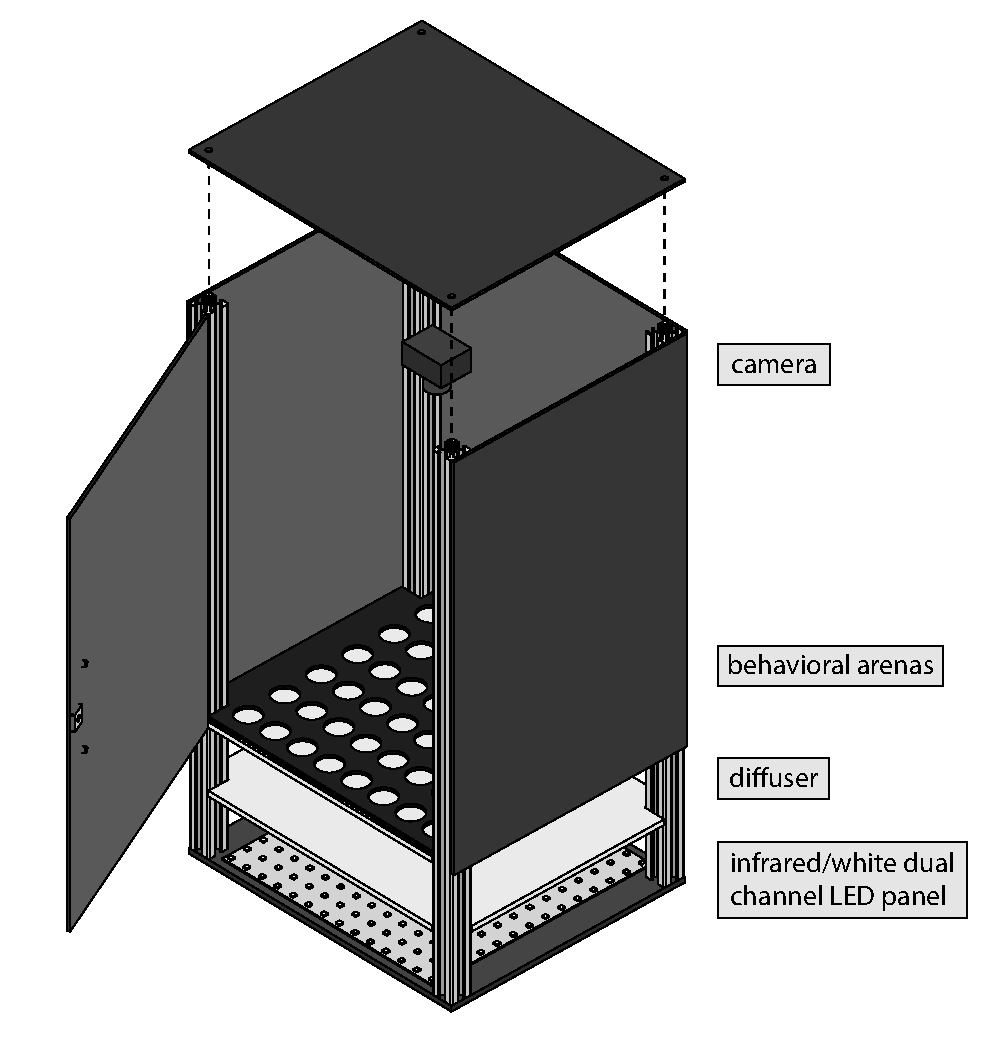
\includegraphics[width=0.5\textwidth]{images/Hardware Setup/Tracking box/behavioral_box_isometric_painted_labels.pdf}
		\caption*{\footnotesize {\textit{figure 2.1} - Sample tracking platform constructed from aluminum rails and acrylic plastic. Backlit behavioral arenas and opaque walls enhance ROI contrast and reduce imaging noise.}}
	\end{center}
\end{figure}

In addition to walls, use clear sanded plastic, diffuser film, or paper either between the illumination source and behavioral arenas or on the floor of the arenas themselves to diffuse the light source. Having a sanded or matte finish on all surfaces inside of the tracking box can also help reduce reflections and glares inside the box.


\hypertarget{arenasection}{\subsection{Individual behavioral arenas}}

MARGO ROI setting can operate in two different modes: \textit{automatic} and \textit{grid} modes. Choosing appropriate individual behavioral arenas will be dependent on the  ROI detection mode used. Automatic detection mode works by finding bright regions of the image that are all roughly the same size. This means that ideal behavioral arenas used for automatic ROI detection are backlit, transparent areas separated by opaque areas in between. Sample arena construction for automatic detection is shown below in fig. 5.

\begin{figure}[h!]
	\begin{center}
		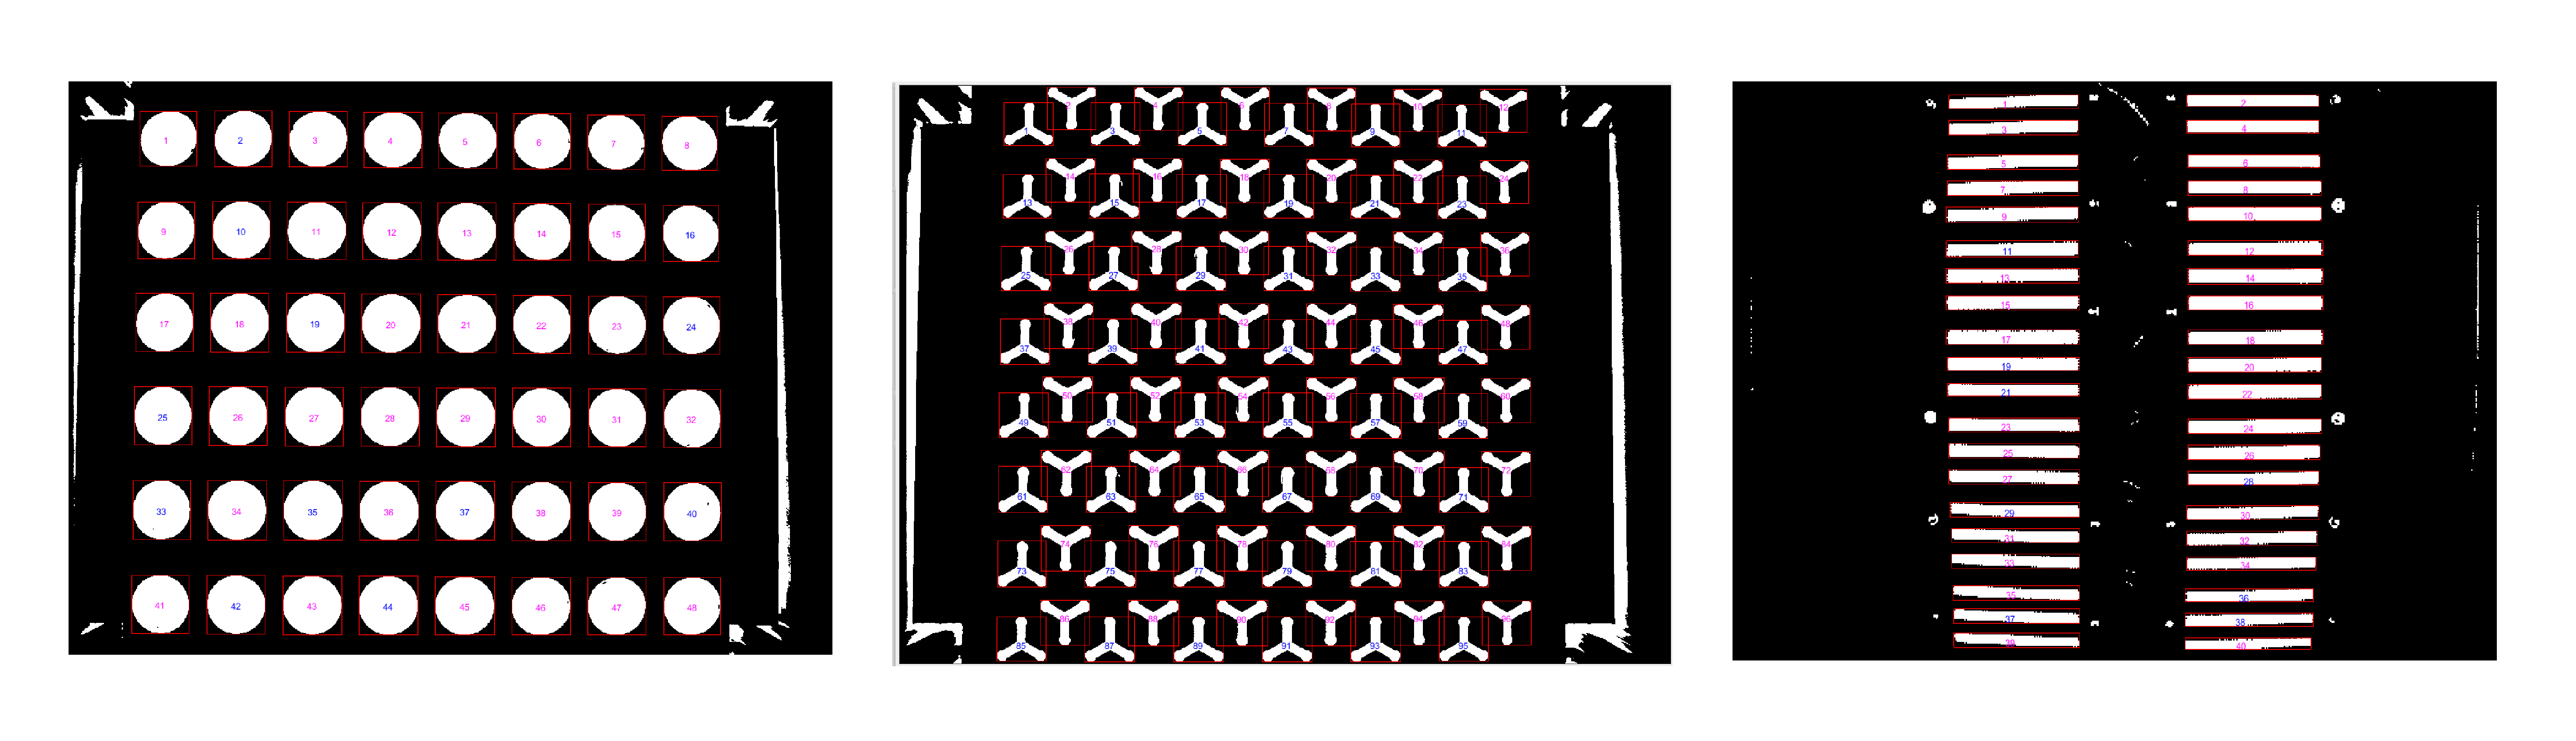
\includegraphics[width=0.95\textwidth]{images/Hardware Setup/Behavioral Arenas/autoROI_detection.pdf}
		\caption*{\footnotesize {\textit{figure 2.2.1} - Sample images of automatic ROI detection.}}
	\end{center}
\end{figure}

Grid detection mode works only on the assumption that ROIs will be arranged in regularly spaced rows and columns. The user is prompted to draw and adjust the position of one or more grids of any arbitrary dimensions to specify ROIs. This means that behavioral arenas can be anything with stereotyped dimensions. Wellplates of any dimensions make ideal behavioral arenas for grid mode detection. Grid mode also works well with linear arrays of tunnels. Sample arena constructions for grid detection mode are shown below in fig. 6.

\begin{figure}[h!]
	\begin{center}
		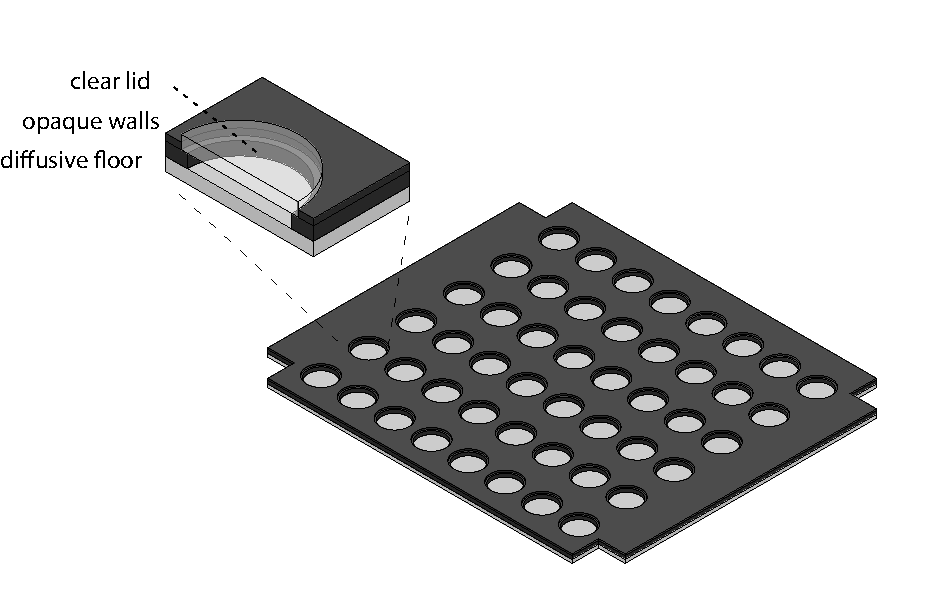
\includegraphics[width=0.5\textwidth]{images/Hardware Setup/Behavioral Arenas/circular_arenas.pdf}
		\caption*{\footnotesize {\textit{figure 2.2.2} - Sample tracking arena constructed from layered, laser cut acrylic. Semi-transparent floors and opaque walls create high-contrast, easily detectable ROIs.}}
	\end{center}
\end{figure}

\hypertarget{illumsection}{\subsection{Illumination}}

Quality illumination is a prerequisite for high-quality tracking. An ideal light source will be evenly diffuse and sufficiently bright. Because MARGO uses a single tracking threshold for the entire field of view of the camera, even illumination is the top priority for an illumination source. MARGO can correct for uneven brightness, but having an even illumination source will ensure that the quality of tracking is equally good in all parts of the cameras field of view. Any illumination source bright enough to saturate the camera is sufficiently bright for tracking.

We perform all of our tracking with infrared light. Using an infrared light source and longpass filter on the camera has the dual benefit of reducing sensitivity of the tracking to perturbation by most external light sources (not sunlight) and allowing for independent control of visible light sources to deliver stimuli not visible to the camera. An affordable example of two color channel LED light panels configured with white and infrared LEDs can be found \href{https://www.knema.com/led-modules.html}{here}. Alternatively, LCD backlight panels can provide a ready-made solution to bright, even illumination.

\hypertarget{camconfig}{\subsection{Camera configuration}}

MARGO has built-in tools to automatically detect and configure any camera visible to MATLAB. The appropriate configuration for your camera will largely depend on your particular experiment. Camera customization features are accessible under the "Hardware" menu bar. But before configuring the camera in MARGO, ensure that the camera and camera lens are properly setup for tracking. The following are good guidelines for configuring your camera:

\begin{itemize}
	\itemsep0em 
	\item Aperture opened enough that ROIs are nearly saturation
	\item Lens maximally zoomed to reduce lens fisheye
	\item Lens focused on ROIs
	\item Camera rigidly fixed to a camera mount
\end{itemize} 

\hypertarget{camdetect}{\subsubsection{camera detection}}

Camera support in MARGO is built on MATLAB's Image Acquisition Toolbox. Before a camera can be detected by MARGO, the associated the associated MATLAB camera adaptors must first be installed. The appropriate adaptor to install will depend on the camera manufucturer. See MATLAB's tutorial for complete instructions on \href{https://www.mathworks.com/help/imaq/installing-the-support-packages-for-image-acquisition-toolbox-adaptors.html}{installing MATLAB camera support packages}.

Once the camera adaptors are installed, a list of available cameras and camera modes should auto-populate upon launching MARGO. The list available cameras can be refreshed under the hardware menubar. 

\hypertarget{cammodes}{\subsubsection{camera modes}}

MARGO will automatically detect available camera modes for operating at different pixel resolutions and color bit depths. The tracking is designed to work with 8-bit color depth because most tracking operations are performed on binary images. It is also strongly recommended that monochromatic cameras are used. By default, MARGO only tracks the green color channel of RGB images.

\hypertarget{camsettings}{\subsubsection{camera settings}}

Camera properties such as exposure time, shutter speed, gain, and frame rate can be adjusted through \textit{camera settings} under the \textit{Hardware} menu bar. Because the configurable settings are specific to each device, the properties that can be adjusted here will depend on your camera. Many cameras have modes to automatically adjust the camera exposure time, shutter speed, frame rate, gain or focus in real time. These modes are also often enabled by default, which may be good for many applications but is highly problematic for tracking. Constantly fluctuating images will introduce a lot of noise into the tracking due to the sensitivity of difference image to even minor changes from frame to frames.

To adjust camera settings, first initiate \textit{preview camera} and leave it running to get feedback on the settings as they change. Select \textbf{\textit{Hardware} $>$ \textit{Camera} $>$ \textit{camera settings}} to open the camera settings window. Keep in mind that the available settings and names of each property will be dependent on the camera. From the settings menu:

\begin{itemize}
	\itemsep0em 
	\item Ensure that any automatically adjust fields are set to "off" or "manual"
	\item Adjust exposure and shutter speeds until the preview is just below saturation
	\item Set max frame rate (target acquisition rate can be set lower in tracking parameters)
	\item Close window to save settings
\end{itemize} 

\section{Starting a New Experiment}

Before running any experiment, MARGO must go through a simple setup that follows the workflow shown in fig. 1. MARGO's user interface enforces this workflow by progressively enabling downstream controls as each sequential step is completed. To access the next step in the workflow, the user must complete the preceding step. Keep in mind that \hyperlink{saveprofile}{loading a custom profile} will allow many of these steps to be skipped and substantially reduce the time needed to setup a new experiment.

\subsection{Confirm camera and camera mode}

The only control panels enabled by default are camera and illumination (not covered here). The user must minimally select a camera, image resolution, and data output format from the drop down menus. Once selected, \textit{confirm settings} to initialize the camera. At this point, it is also a good to preview the camera and adjust any other camera settings if necessary. Because the tracking and ROI thresholds selected in the downstream steps can be sensitive to changes in exposure, shutter speed, and gain, it is strongly recommended that these settings are \hyperlink{camsettings}{manually configured} before continuing.

\hypertarget{roidetect}{\subsection{ROI detection}}

A region of interest (ROI), is a static location in the camera's field of view that tells MARGO where to expect tracked objects. All movement or changes in the image outside of the ROIs will be untracked. The software is forgiving of setting ROIs in regions without a tracked objects since ROIs with little or no movement by filtering traces in those ROIs, but is unforgiving of failing to set an ROI over a tracking target. It is therefore important that ROIs are set properly before the tracking begins. ROI detection in MARGO comes in two flavors: \textit{auto} and \textit{grid} detection modes. As the name suggests, \textit{auto} mode is essentially instantaneous and easy, but requires your ROIs and imaging setup to meet particular conditions. This mode is enabled by default. On the other hand, \textit{grid} mode tolerates greater variability in ROI and imaging conditions but requires the user to draw and position one or more ROI grids over the image. ROI detection modes can be switched under \textbf{\textit{Tracking} $>$ \textit{tracking parameters} $>$ \textit{ROI detection}}.


\textbf{auto mode}

Automatic ROI detection works by finding a threshold value that separates bright regions of the image from a dark background. Before applying the threshold, MARGO first attempts to correct for in vignetting or global unevenness in the illumination. Images commonly tend to be brighter in the center and dimmer at the edges, correcting this unevenness makes it easier to find a single threshold value that will cleanly separate all ROIs in the field of view from the background.

To run automatic ROI detection, select \textbf{\textit{detect ROIs}} and adjust the ROI threshold slider until the ROIs are cleanly separated from the background. Displayed ROI numbers and bounding boxes show the automatically assigned identity of each ROI in the image and its boundaries. A vertical orientation indicated by font color will also be assigned to each ROI. This is useful for ROIs with a clear vertical assymetry such as the ones shown in \textbf{fig 3.2.1}. Orientation can largely be ignored for ROIs without assymetry.

The following steps may help in cases where auto mode detection either fails to pick up or inaccurately identifies one or more ROIs:

\begin{itemize}
	\itemsep0em 
	\item increase the threshold if it incorrectly assigns identities to non-ROIs
	\item decrease the threshold if fails to detect real ROIs
	\item ensure nothing dark or opaque bisects any ROIs
	\item use \hyperlink{vignettecorrection}{manual vignette correction} if uneven illumination causes ROI dropping at the edges of the camera field of view
	\item \hyperlink{ROIediting}{manually edit} individual ROIs if needed
\end{itemize}

\begin{figure}[h!]
	\begin{center}
		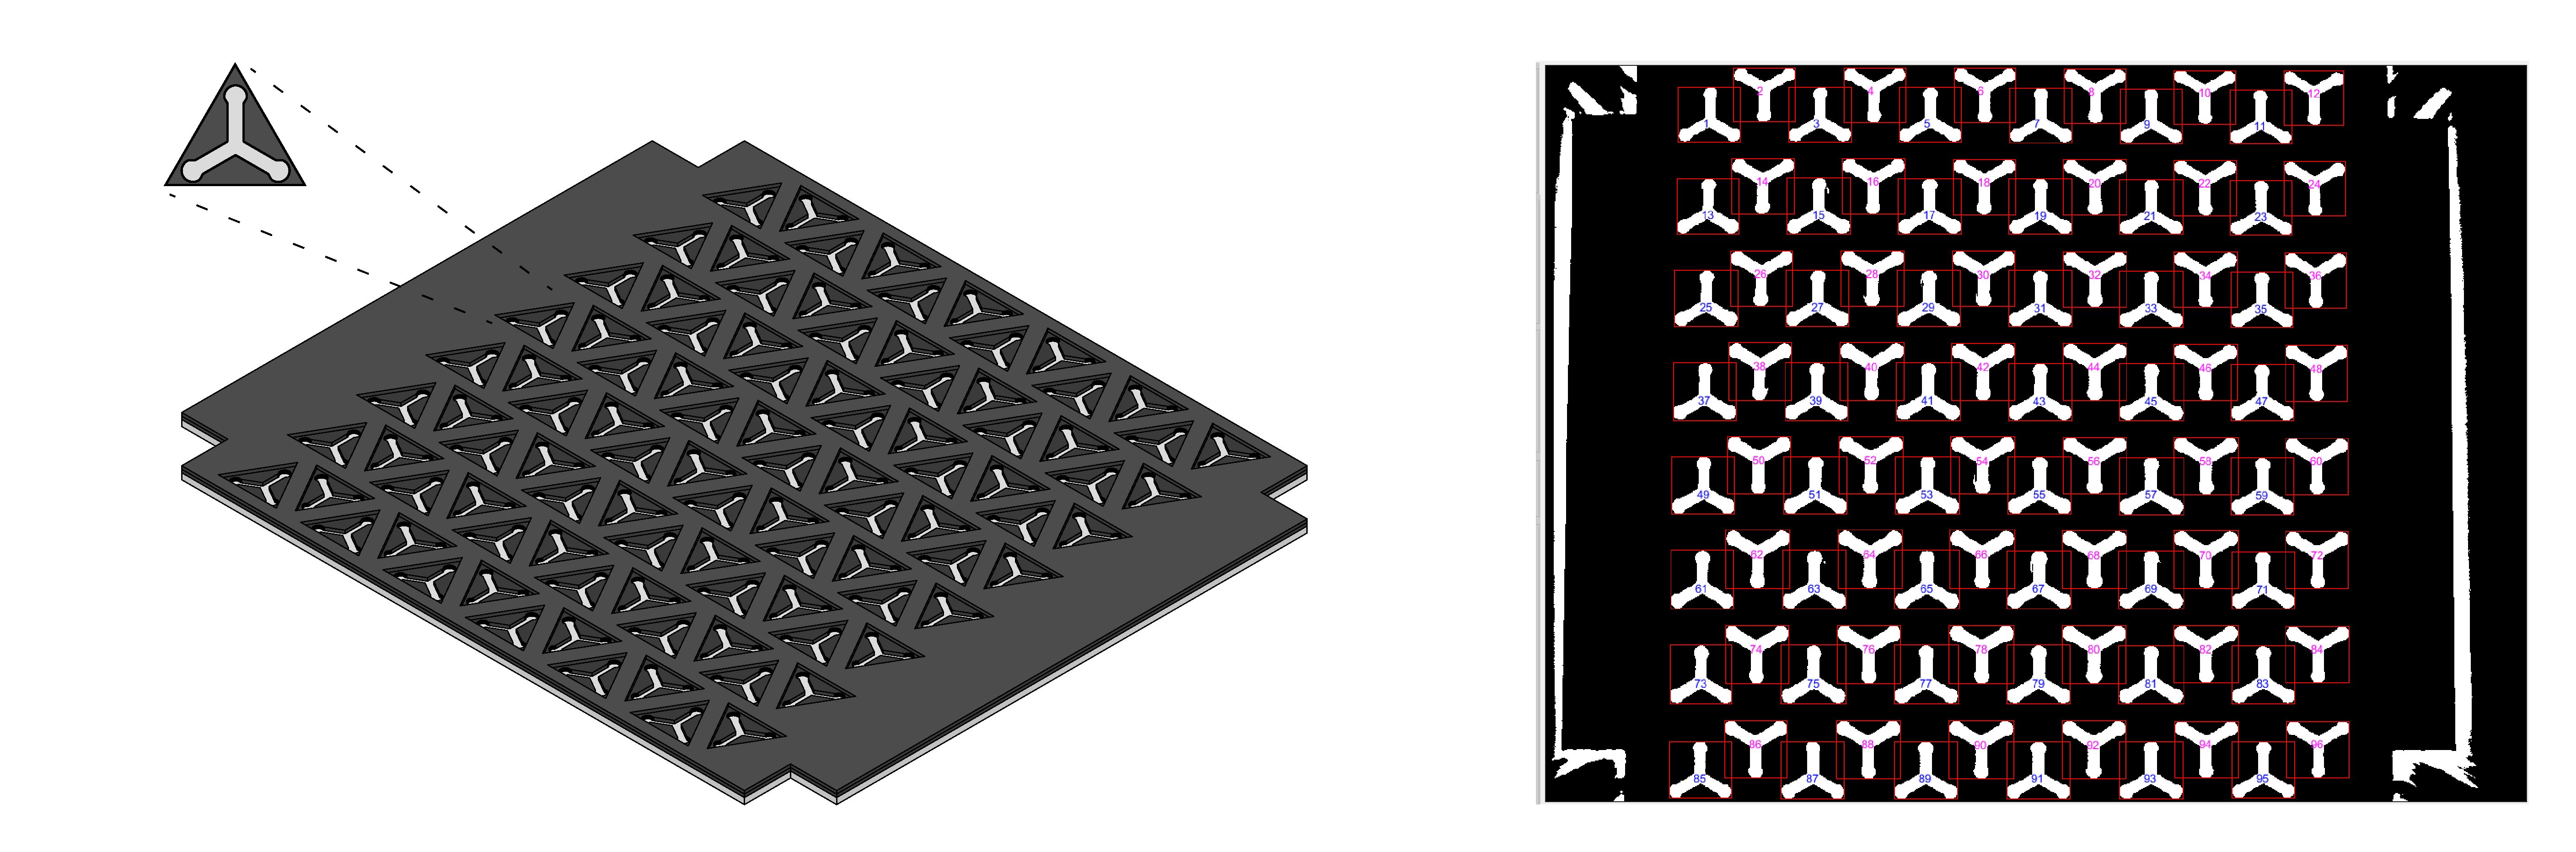
\includegraphics[width=0.85\textwidth]{images/Starting a New Experiment/ymaze_96mazes_isometric.pdf}
		\caption*{\footnotesize {\textit{figure 3.2.1} - Sample schematic (left) and ROI detection (right) of an arena optimized for automatic detection. Non-grid structure of arenas makes it unsuitable for grid detection mode. Automatic ROI detection records vertical asymmetry of ROIs. In a Y-shaped arena, recording the orientation makes it easy to infer endpoints of the maze arms.}}
	\end{center}
\end{figure}

\textbf{grid mode}

Grid mode ROI detection avoids the need for using imaging tricks to assign ROIs but requires a little user input to make assignments. This mode also makes the assumption that boundaries between ROIs can be drawn in a regular grid-like structure.

After starting grid-based detection by selecting \textit{detect ROIs}, the user interface controls will be temporarily disabled as it waits for the user to drag and drop a new grid into the imaging window. A grid settings user panel will appear with options to add and remove grids as well as change the dimensions of each grid. Once a grid is placed in the imaging window, customize the grid by repositioning corners or editing the number of rows and columns. The ROI bounds displayed in the imaging window show the enclosed space in which a centroid will be assigned to a particular ROI. The bounds should be positioned such that they fall in the space arenas. New grids can be added or removed at any time by selecting the + and - controls. Multiple grids allows several trays to be imaged simultaneously by the same camera. This works particularly well when imaging multiple well plates at the same time. Once finished editing grids, select \textit{Accept} to save the ROI positions.

\vspace*{.75cm}
\begin{figure}[h!]
	\begin{center}
		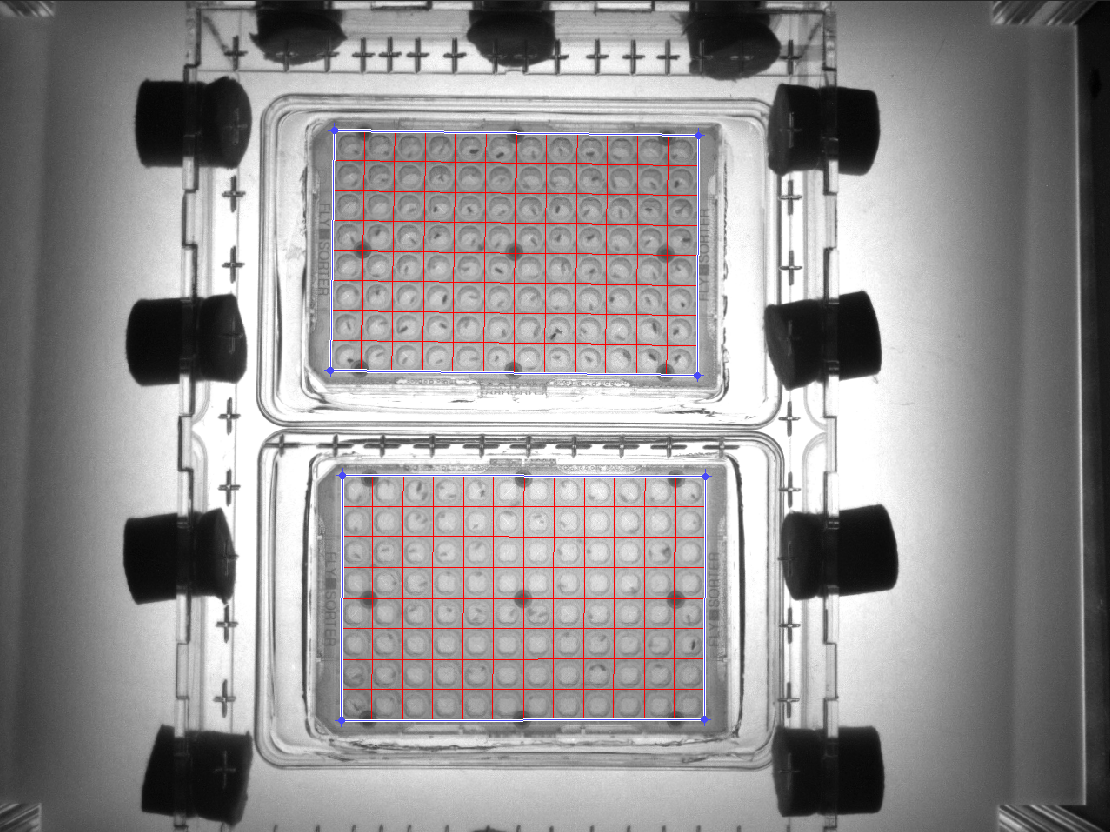
\includegraphics[width=0.5\textwidth]{images/Hardware Setup/Behavioral Arenas/ROIs_detected_1.png}
		\caption*{\footnotesize {\textit{figure 3.2.2} - Grid detection mode captures regularly arrayed and low-contrast ROIs.}}
	\end{center}
\end{figure}


\subsection{Background referencing}

Once ROI locations are set, MARGO creates a background reference image to keep track of the frame to frame differences between the current frame and the background image. MARGO uses periodic sampling of the background throughout tracking to constantly update the background appearance, but a reference must first be initialized before tracking can begin.  Because the arenas are not actually empty when this reference is created, MARGO takes snapshots of each ROI separately any time a tracked individual has moved far enough away from any position where a previous snapshot was taken. A median image is computed for each ROI separately and then combined into a single master reference for entire field of view. Initializing a relatively accurate reference \textit{very important} because it allows for accurate noise profiling, which is essential for robust tracking.

Select \textbf{\textit{initialize reference}} to begin referencing. The imaging window will display a thresholded difference image between the reference and the current frame. Because the reference is first initialized to a sample image at the start of referencing, the image should be largely blank at first but begin to populate with individuals as they begin to move. New samples of each ROI will be progressively collected as individuals move around in each ROI. Circular indicators to the upper left of each ROI will progress from purple to green as more references are taken for each ROI, with green indicating referencing complete for a given ROI. Adjust the tracking threshold until pixel noise is largely absent from the thresholded image. Select \textit{Accept} on the tracking threshold slider to set the reference image. \textit{Note:} Rougly half or more of the ROIs at green should be sufficient to proceed to sampling noise statitics.

\subsection{Noise profiling}

Difference imaging is extremely sensitive to even minor changes between the background reference and the current frame. For that reason, minor pertubations to the imaging such ambient vibrations over long time scales or acute pertubations such as bumping tracking box can drastically increase the noise in tracking. MARGO samples the distribution of above threshold pixels during a sample, clean tracking period of one hundred frames so that it can constantly monitor the quality of and counter any deterioration in the difference image. For this approach to work, the distribution collected during this period must be a relatively accurate representation of what it should look during the rest of the experiment.

Select \textbf{\textit{confirm tracking}} to begin sampling. The tracking threshold can be adjusted up or down to bias sampling to be either more or less sensitive to noise during tracking. Noise sampling tips:

\begin{itemize}
	\itemsep0em
	\item Try to get at least half of all ROIs completely referenced during the previous step
	\item Slightly lower the tracking threshold if too few individuals are showing above the difference image
	\item Obtain more accurate noise profiling or further lower the tracking threshold during sampling if noise threshold reference reset is constantly triggered during tracking
\end{itemize}

\subsection{Experiment settings}

With the tracking setup complete, all that remains is to select the experiment to be run and, if necessary adjust a few settings before beginning tracking.

\subsubsection{select experiment}

The experiment selection determines which experiment and data processing protocols to execute once tracking begins. If you only want to record centroid coordinates and time stamps, select \textit{Basic Tracking} from the dropdown menu and move to the next step. MARGO was designed not only to record basic tracking data, but to run a suite of experimental protocols. Those protocols differ in the raw data they record as well as their hardware control schema and behavioral metrics recorded. Users can define their own \hypertarget{customexperiment}{custom experiments} or select from a list of pre-defined protocols. More detailed explanations of the pre-defined experiments in MARGO see the \href{https://www.google.com}{
original MARGO publication}.

\subsubsection{parameters}

If necessary, adjust the duration of tracking in hours, the number of reference samples per minute, and the number of reference samples to collect per ROI. Depending on the selected experiment, additional customizable may be available under \textit{experiment parameters}. Keep in mind not all protocols, including \textit{Basic Tracking} will have any additional parameters to adjust.

\subsubsection{labels}

Select \textit{labels} to attach meta data to any particular range of ROIs. By default, MARGO has fields for recording genetic strain, sex, treatment condition, ID numbers, Day of testing, tracking box, tracking arena/plate, and any additional comments. To append labels, enter a range or ROIs the label applies to, fill in the labels, and select \textit{Accept}. Distinct categories can be entered in subsequent rows. \textit{Note:} MARGO will auto-generate a file label from the first row of entries.
 
\subsubsection{save path}

Browse to a parent directory for the MARGO output. MARGO will auto-generate a new directory within the chosen save path with the time stamp and label information for the experiment where it will save all raw and processed data. 

\hypertarget{saveprofile}{\subsection{Save your settings - \textit{recommended}}}

Before starting the experiment, it is \textit{strongly} recommended to save a profile for the current configuration of \textit{MARGO}. By loading a saved configuration profile in the future, you will avoid having to do any parameter configuration. Only information such as the ROI positions and reference image that is unique to each instance of tracking will not be saved. Saving a profile not only substantially simplifies the setup process, but also ensures consistency that will make it easier to compare recordings across sessions.

To save a new profile, select \textit{File} $>$ \textit{save a new preset}. A profile can be loaded at any time, but because presets contain information about camera configuration, it will be necessary to re-initialize the camera anytime a new preset is loaded.

\newpage
\section{Running Analysis}

MARGO will execute an analyze file for the  accompanying run file upon finishing tracking. Processing times can vary greatly depending on your computer and the size of the raw data files. Once analysis is complete, the user will be given the option to view raw centroid data. At this point, the \emph{\textit{ExperimentData}} master can be loaded into the MATLAB workspace by copying and executing the command printed to the command window or by browsing to the save directory and manually loading the file.

Users may wish to try processing the data multiple different ways or set optional  processing flags or parameters. For this reason, MARGO has functions for re-processing data files, repairing broken references to raw data files, and setting optional processing flags.

The simplest way to get started is the \textbf{\textit{analyze\_multiFile}} function. This function allows the user to browse and select a parent directory containing all files to be reprocessed. Once a parent directory is selected, the function will search recursively through all directories underneath for any .mat files. An optional keyword can be provided to restrict the query to file names containing the keyword argument. The \textit{\textit{ExperimentData}.Name} property is used to query and execute to the accompanying analyze file for each file sequentially. This means that \textit{\textit{ExperimentData}} files of many different types can be processed together in batches. The following name-value pairs can be set to customize the analysis:

\begin{figure}[h!]
	\vspace*{0.75cm}
	\begin{center}
		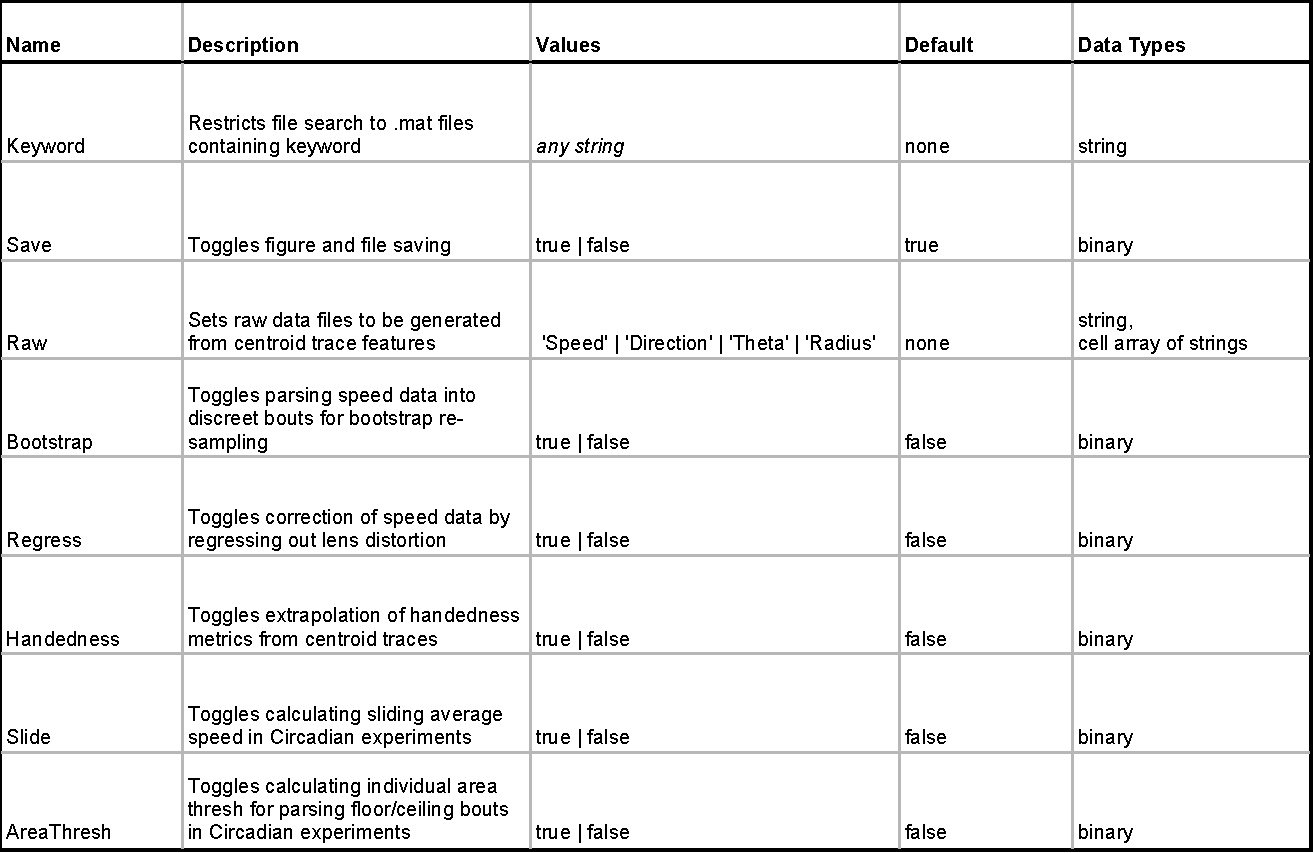
\includegraphics[width=0.95\textwidth]{images/analysis/namevalue.pdf}
		\caption*{\footnotesize {\textit{table 4.1} - Processing name-value pairs for analyze\_multiFile}}
	\end{center}
\end{figure}

\newpage
\section{Data Output}

Data is output from MARGO in three phases. Once the play button is pushed, MARGO generates and saves a .mat file with all meta data during initialization of the experiment. During tracking, MARGO writes raw data fields to the hard drive. Once tracking is finished, a round of protocol-specific, automatic data processing is performed to calculate metrics for higher level features of the raw data.

\subsection{Raw data}

Raw data is saved frame by frame to binary data files located in the subdirectory under the user-defined save path. Each tracked field is saved independently to its own file. The data can be read directly into MATLAB or accessed indirectly through memmaps in the \textit{ExperimentData} object. The simplest way to access the data quickly is through the automatically generated memory maps. However, the binary data files can be accessed via MATLAB's \textit{fread} function. If attempting to access the raw data directly, keep in mind that the data must be read in the correct precision and dimensions. In addition to the ability to record user-defined raw data, MARGO can record the following pre-defined raw data fields: \textit{centroid},\textit{ inter-frame interval (ifi)}, \textit{area}, \textit{orientation}, and \textit{speed}.

\subsection{Master Data Container (ExperimentData)}

A single object, \textit{ExperimentData}, allows the user to access all raw and processed data output. The master data container is saved to a .mat file in an auto-generated, time-stamped directory under the save directory. The \textit{ExperimentData} master data container can be easily loaded into MATLAB and is a convenient way to browse and manipulate all the data.  \textit{ExperimentData} contains four core properties:

\begin{enumerate}
	\item Data - Contains custom \textit{RawDataField} objects which contain meta data about the raw data files and allow the user to dynamically access raw data from the files.
	\item Meta - Contains experiment meta data (e.g. ROIs, background references, labels, file path information).
	\item Parameters - Contains all experimental parameters and their values.
	\item Hardware - Contains hardware objects (e.g. cameras, displays) and associated meta data.
\end{enumerate}

See \hyperlink{expmttable}{table 5.2} for a complete details of the contents of the \textit{ExperimentData} object.

\subsubsection{Experiment meta data}

All meta data from the experiment is saved to the master data container during initialization of tracking. By default, MARGO records the following meta data:


\begin{multicols}{2}
	\begin{itemize}
		\itemsep0em
		\item time, date, and duration
		\item ROI position and dimensions
		\item label meta data
		\item camera and other hardware settings
		\item referencing and tracking parameters
		\item imaging noise statistics
		\item raw data file paths, format, and dimensions
		\item protocol specific parameters
	\end{itemize}
\end{multicols}


\subsubsection{Memory mapped raw data}

Raw data files can be accessed and de-accessed through the \textit{ExperimentData} master data container through the use of a custom \textit{RawDataMap} object. These objects are built on top of MATLAB's \href{https://www.mathworks.com/help/matlab/ref/memmapfile.html}{memory maps}, for efficient access of large binary data files. Although MARGO has a much lighter data footprint than raw video data, raw data files can still be cumbersome, or impossible to hold in memory. Because MARGO can efficiently track and record activity from thousands of individuals over very long timescales, raw data files can easily exceed several gigabytes in size. For this reason, raw data is dynamically read from the hard drive to avoid \textit{out of memory} errors. Mapped raw data can be dynamically accessed under \textit{expmt.data.(raw field name).raw} like a normal MATLAB array. For example, centroid data can be accessed under \textbf{expmt.data.centroid.raw} and is formated as $ M x N x P$ matrix where M = number of frames, N = 2 (x,y), and P = number of ROIs. If we wanted to assign the centroid coordinates for ROI \#10 for the entire length of the experiment to temporary variables, we could call:

\begin{center}
	 \textit{x = expmt.data.centroid.raw(:, 1, 10);}\\
	\textit{y = expmt.data.centroid.raw(:, 2, 10)};
\end{center}

\subsubsection{auto-processed centroid features}

When tracking is finished, MARGO can be configured to run a protocol-specific, data-processing script to perform data pre-processing or analysis. All tracking protocols in MARGO minimally record centroid position and inter-frame interval. As examples of higher level features, MARGO uses post-processing to generate measures of:  \textit{individual activity},  \textit{locomotor handedness}, and  \textit{stimulus evoked behaviors}.

\subsection{Figures}

Depending on the selected tracking protocol, MARGO may output figures during post-processing. All figures are saved to an auto-generated \textit{figures} directory under the user specified save location. The figure directory is saved to \textit{expmt.meta.path.fig} in the master data container.


\subsubsection{Raw Trace Browser}

Users will be prompted to browse raw trace data upon tracking completion. Select \textbf{\textit{browse traces}} to open a simple GUI for plotting centroid data. Traces from any \textit{\textit{ExperimentData}} master data container can be browsed at anytime by loading the .mat file and running \textbf{\textit{plotTraces(\textit{ExperimentData})}} from the MATLAB command line.

\vspace*{0.75cm}
\begin{figure}[h!]
	\begin{center}
		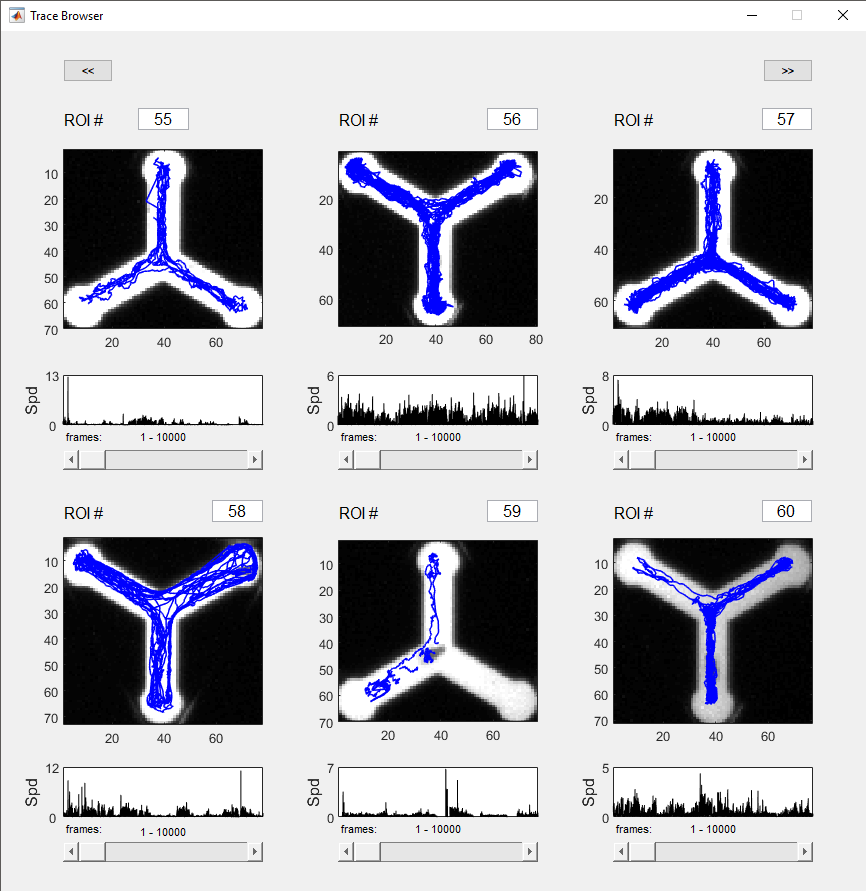
\includegraphics[width=0.6\textwidth]{images/outputs/trace_browser.png}
		\caption*{\footnotesize {\textit{figure 4.3.1} - Raw trace browser utility can be used to view raw centroid traces. Plot traces for an \textit{\textit{ExperimentData}} master data container by running \textit{plotTraces(\textit{ExperimentData})}}}
	\end{center}
\end{figure}

\newpage
\hypertarget{\textit{ExperimentData}table}{}
\begin{figure}[h!]
	\begin{center}
		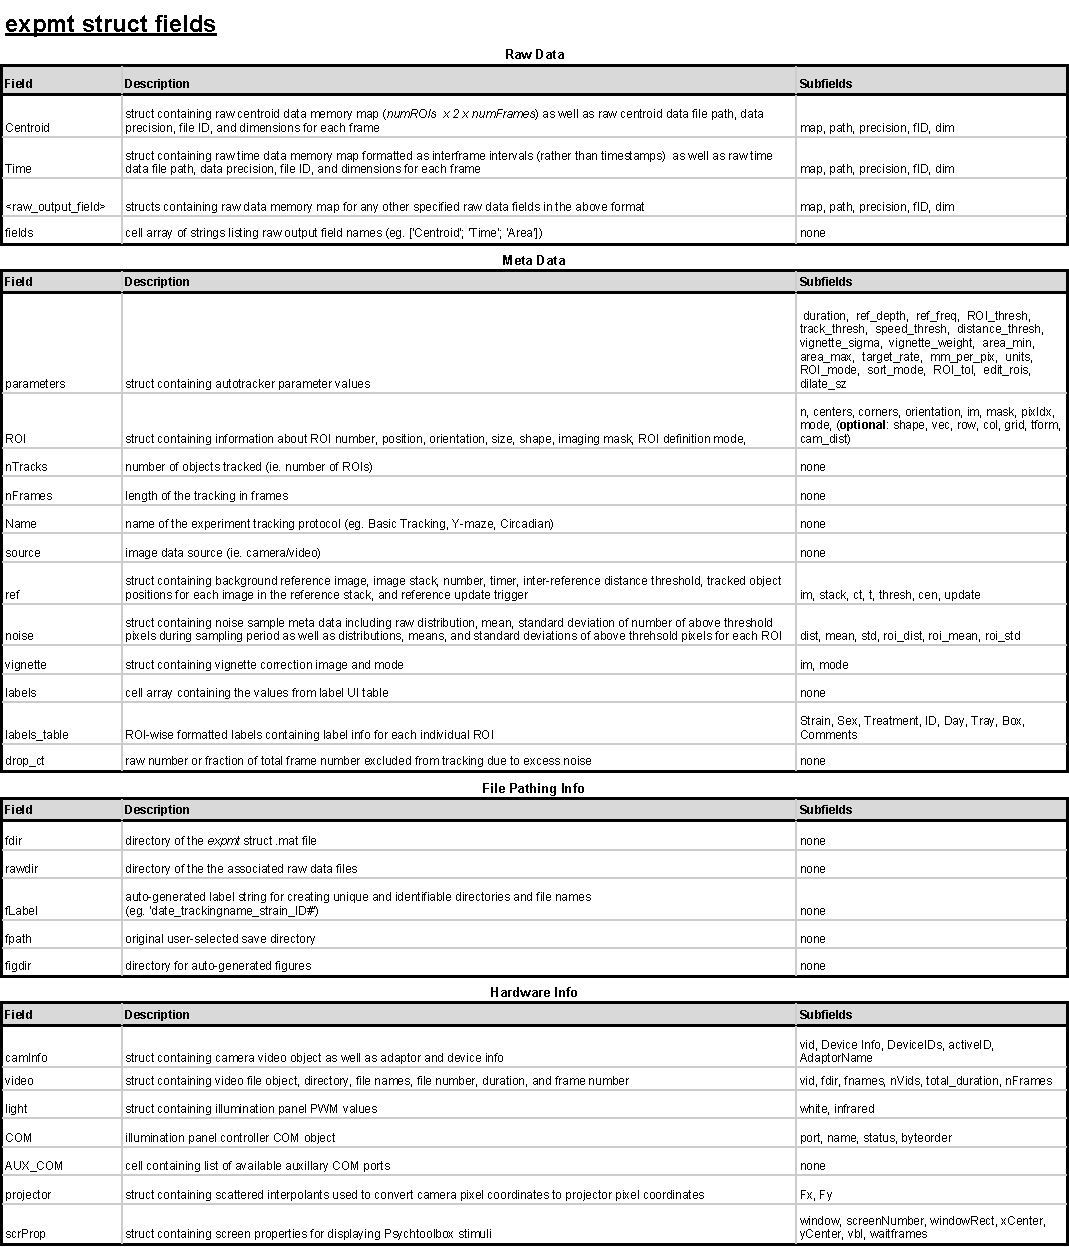
\includegraphics[width=1\textwidth]{images/outputs/expmt_fields.pdf}
		\caption*{\footnotesize {\textit{table 4.1} - Processing name-value pairs for analyze\_multiFile}}
	\end{center}
\end{figure}


\newpage
\section{Advanced Tracking Features}

MARGO understands that the setup and goals of tracking can vary greatly from instance to instance. For that reason, many tools have been included to offer flexibility and customization in how ROIs and centroids are tracked, sorted, and measured.

\subsection{Tracking parameters}

Many of tracking parameters are used to track, identify, or sort ROIs and tracked objects. These parameters can be adjusted under \textit{Tracking} $>$ \textit{tracking parameters}.

\begin{itemize}
	\itemsep1em
	\item \textbf{speed threshold} - maximum allowed distance traveled per second. Each update in an object's position is time-stamped. Every frame, MARGO starts with unassigned blobs in a difference image. To assemble blob positions into traces over time, tracked objects are assigned to an ROI. The speed threshold excludes centroids in any given frame that have moved too far from the last recorded centroid for the paired ROI. This parameter helps prevent the centroid from jumping to pixel. \textit{Note:} toggling the speed threshold radio button after ROI detection and referencing will display a measured rolling average speed and standard deviation for each ROI to help with parameter setting.
	
	\item \textbf{distance threshold} - maximum allowed distance to the center of an ROI. This parameter is used to identify which ROI to assign blob centroids. This parameter is only used when \textit{distance} centroid sort mode is selected. \textit{Note:} toggling the distance threshold radio button will display a circle showing the range of inclusion for each ROI.
	
	\item \textbf{area thresholds} - these parameters set lower and upper bounds that blobs in the threshold image will be tracked. Objects in the image outside of this range are excluded from tracking in the current frame. \textit{Note:} toggling the area threshold radio button after ROI detection and referencing will display a measured rolling average area and standard deviation for each ROI to help with parameter setting. This will also display concentric circles of area equal to the specified bounds.
	
	\item \textbf{vignette gaussian weight} - sets the multiplicative weight of a gaussian mask applied to the entire image during ROI detection. Detecting all ROIs in an image of varying luminance can be challenging. Once MARGO knows which parts of the image are foreground and which are background, a vignette filter can easily be calculated. Before foreground and background are distinguished, some assumptions can help smooth the luminance profile of the image. Many camera lenses and luminance sources create images that are slightly brighter in the center and dimmer at the edges. By default, MARGO assumes a gaussian profile of global luminance in the image and applies a filter to the image to smooth the global luminance. A lower weight will reduce the smoothing applied to the image. \textit{Note:} this parameter is only used during automatic ROI detection and does not apply to \textit{grid mode} detection or object tracking.
	
	\item \textbf{vignette gaussian sigma} - sets the standard deviation of the above vignette correction gaussian as a fraction of the image height. \textit{Note:} this parameter is only used during automatic ROI detection and does not apply to \textit{grid mode} detection or object tracking.
	
	\item \textbf{target acquisition rate} - sets the maximum acquisition rate of tracking in hertz. Adjusting this parameter only ensures that tracking will not exceed this rate. The maximum achievable rate will depend on computer hardware, image resolution, number of objects tracked and centroid sorting mode. For more information on optimizing acquisition rate, see \hyperlink{trackingperformance}{improving tracking performance}. 
	
	\newpage
	\item \textbf{ROI clustering tolerance} - sets the maximum number of standard deviations in vertical distance for adjacent ROIs to be assigned to the same ROI. To automatically assign numbers to ROIs when using \textit{auto} ROI detection mode, MARGO first sorts ROIs by their vertical center of mass and measures the vertical distance between adjacent ROIs. Any pair of ROIs that are within the maximum number of standard deviations of one another are said to belong to the same row. Decreasing this value will make vertical clustering of ROIs more stringent. Increasing the value will cluster ROIs that are more vertically separated into the same row of ROIs. \textit{Note:} this parameter is only used during automatic ROI detection and does not apply to \textit{grid mode} detection or object tracking.
	
	\item \textbf{dilation size} - sets the number of pixels to dilate and erode the threshold image. Dilation and erosion helps fill in gaps between above threshold pixels that, ideally, should belong to the same blob. This is particular helpful in under-illuminated images where tracked individuals are split into multiple nearby blobs. Increasing this value will result in slower tracking speed but will help stitch nearby pixel islands into the same blob. \textit{Note:} set this value to zero to disable dilation and erosion. 
	
	\item \textbf{sort mode} - sets mode by which centroids are assigned to ROIs. \textit{Distance} and \textit{bounds} sorting modes requires centroids to be within the specified distance of the center or fall within the bounds of an ROI, respectively. Centroids not meeting the requirement are not eligible for assignment to that ROI. \textit{Distance} mode is most useful with round shaped ROIs. \textit{Bounds} mode is most useful with elongated ROIs that have an asymmetric width and height. \textit{Note:} bounds sorting mode is automatically employed when grid ROI detection mode is used.
	
	\item \textbf{ROI detection mode} - sets the mode by which ROIs in the camera's field of view are defined. See \hyperlink{roidetect}{ROI detection} for more details on these tracking modes.
\end{itemize}

\subsection{Converting pixel units to mm}

By default MARGO measures distances in pixel units. A tool is included to allow calculating a pixel/millimeter conversion factor by drawing a line over a known distance in the image. To begin, measure the length in mm of any object that will go into the camera's field of view (eg. length of a 96 well plate). Place the object in under the camera and select \textit{Tracking} $>$ \textit{distance scale} to open the conversion tool. Enter the length of the target object in mm in the space provided and select \textit{draw line}. Click and drag in the camera preview window to drag and drop a line along the length of the target object to automatically calculate and store a pixel/mm conversion factor. If necessary, reposition the line end points and select \textit{update} to calculate a new conversion factor. Close the window to save and exit. For accurate measurement, ensure the following:

\begin{itemize}
	\item behavioral platform is perpendicular to the camera
	\item conversion factor is reacquired if the camera adjusted
	\item camera is calibrated to correct for fisheye lens distortion 
\end{itemize}

\subsection{Camera calibration}

Camera parameter objects output by MATLAB's \href{https://www.mathworks.com/help/vision/ug/single-camera-calibrator-app.html}{camera calibrator app} can be used to correct fisheye lens distortion in images. To use camera calibration in MARGO, follow the instructions in MATLAB's tutorial to calculate and export camera parameters to correct images. Save the exported object \texttildelow\textit{MARGO/hardware/camera\_calibration/} in a .mat file. Create the \textit{camera\_calibration} directory if necessary. MARGO will automatically look for camera parameter objects in the specified directory upon initialization. Once the camera parameter object is exported and saved, toggle calibration under \textit{Hardware} $>$ \textit{camera} $>$ \textit{use calibration}.

\subsection{Vignette correction}

Variation in baseline luminance across images can make it difficult to cleanly separate out tracked objects and ROIs with a single threshold value. MARGO uses vignette correction to increase the dynamic range over which objects can be separated from the background. To achieve this, the software employs two different strategies to smooth the baseline illumination of all ROIs in the image. 

\begin{itemize}

\item \textbf{Gaussian correction} is utilized in \textit{auto ROI detection} mode prior to initial detection of ROIs. Uneven illumination occurs most commonly as vignetting (ie. light fall-off) at the edges of image (fig 5.4). MARGO uses the assumption of a gaussian profile of vignetting centered on the image to smooth out the illumination. The width and weighting of the gaussian can be adjusted under \textit{tracking parameters}. Figure 5.4 illustrates how correcting vignetting can allow all ROIs in the image to be cleanly separated from the background.

\begin{figure}[h!]
	\vspace*{0.75cm}
	\begin{center}
		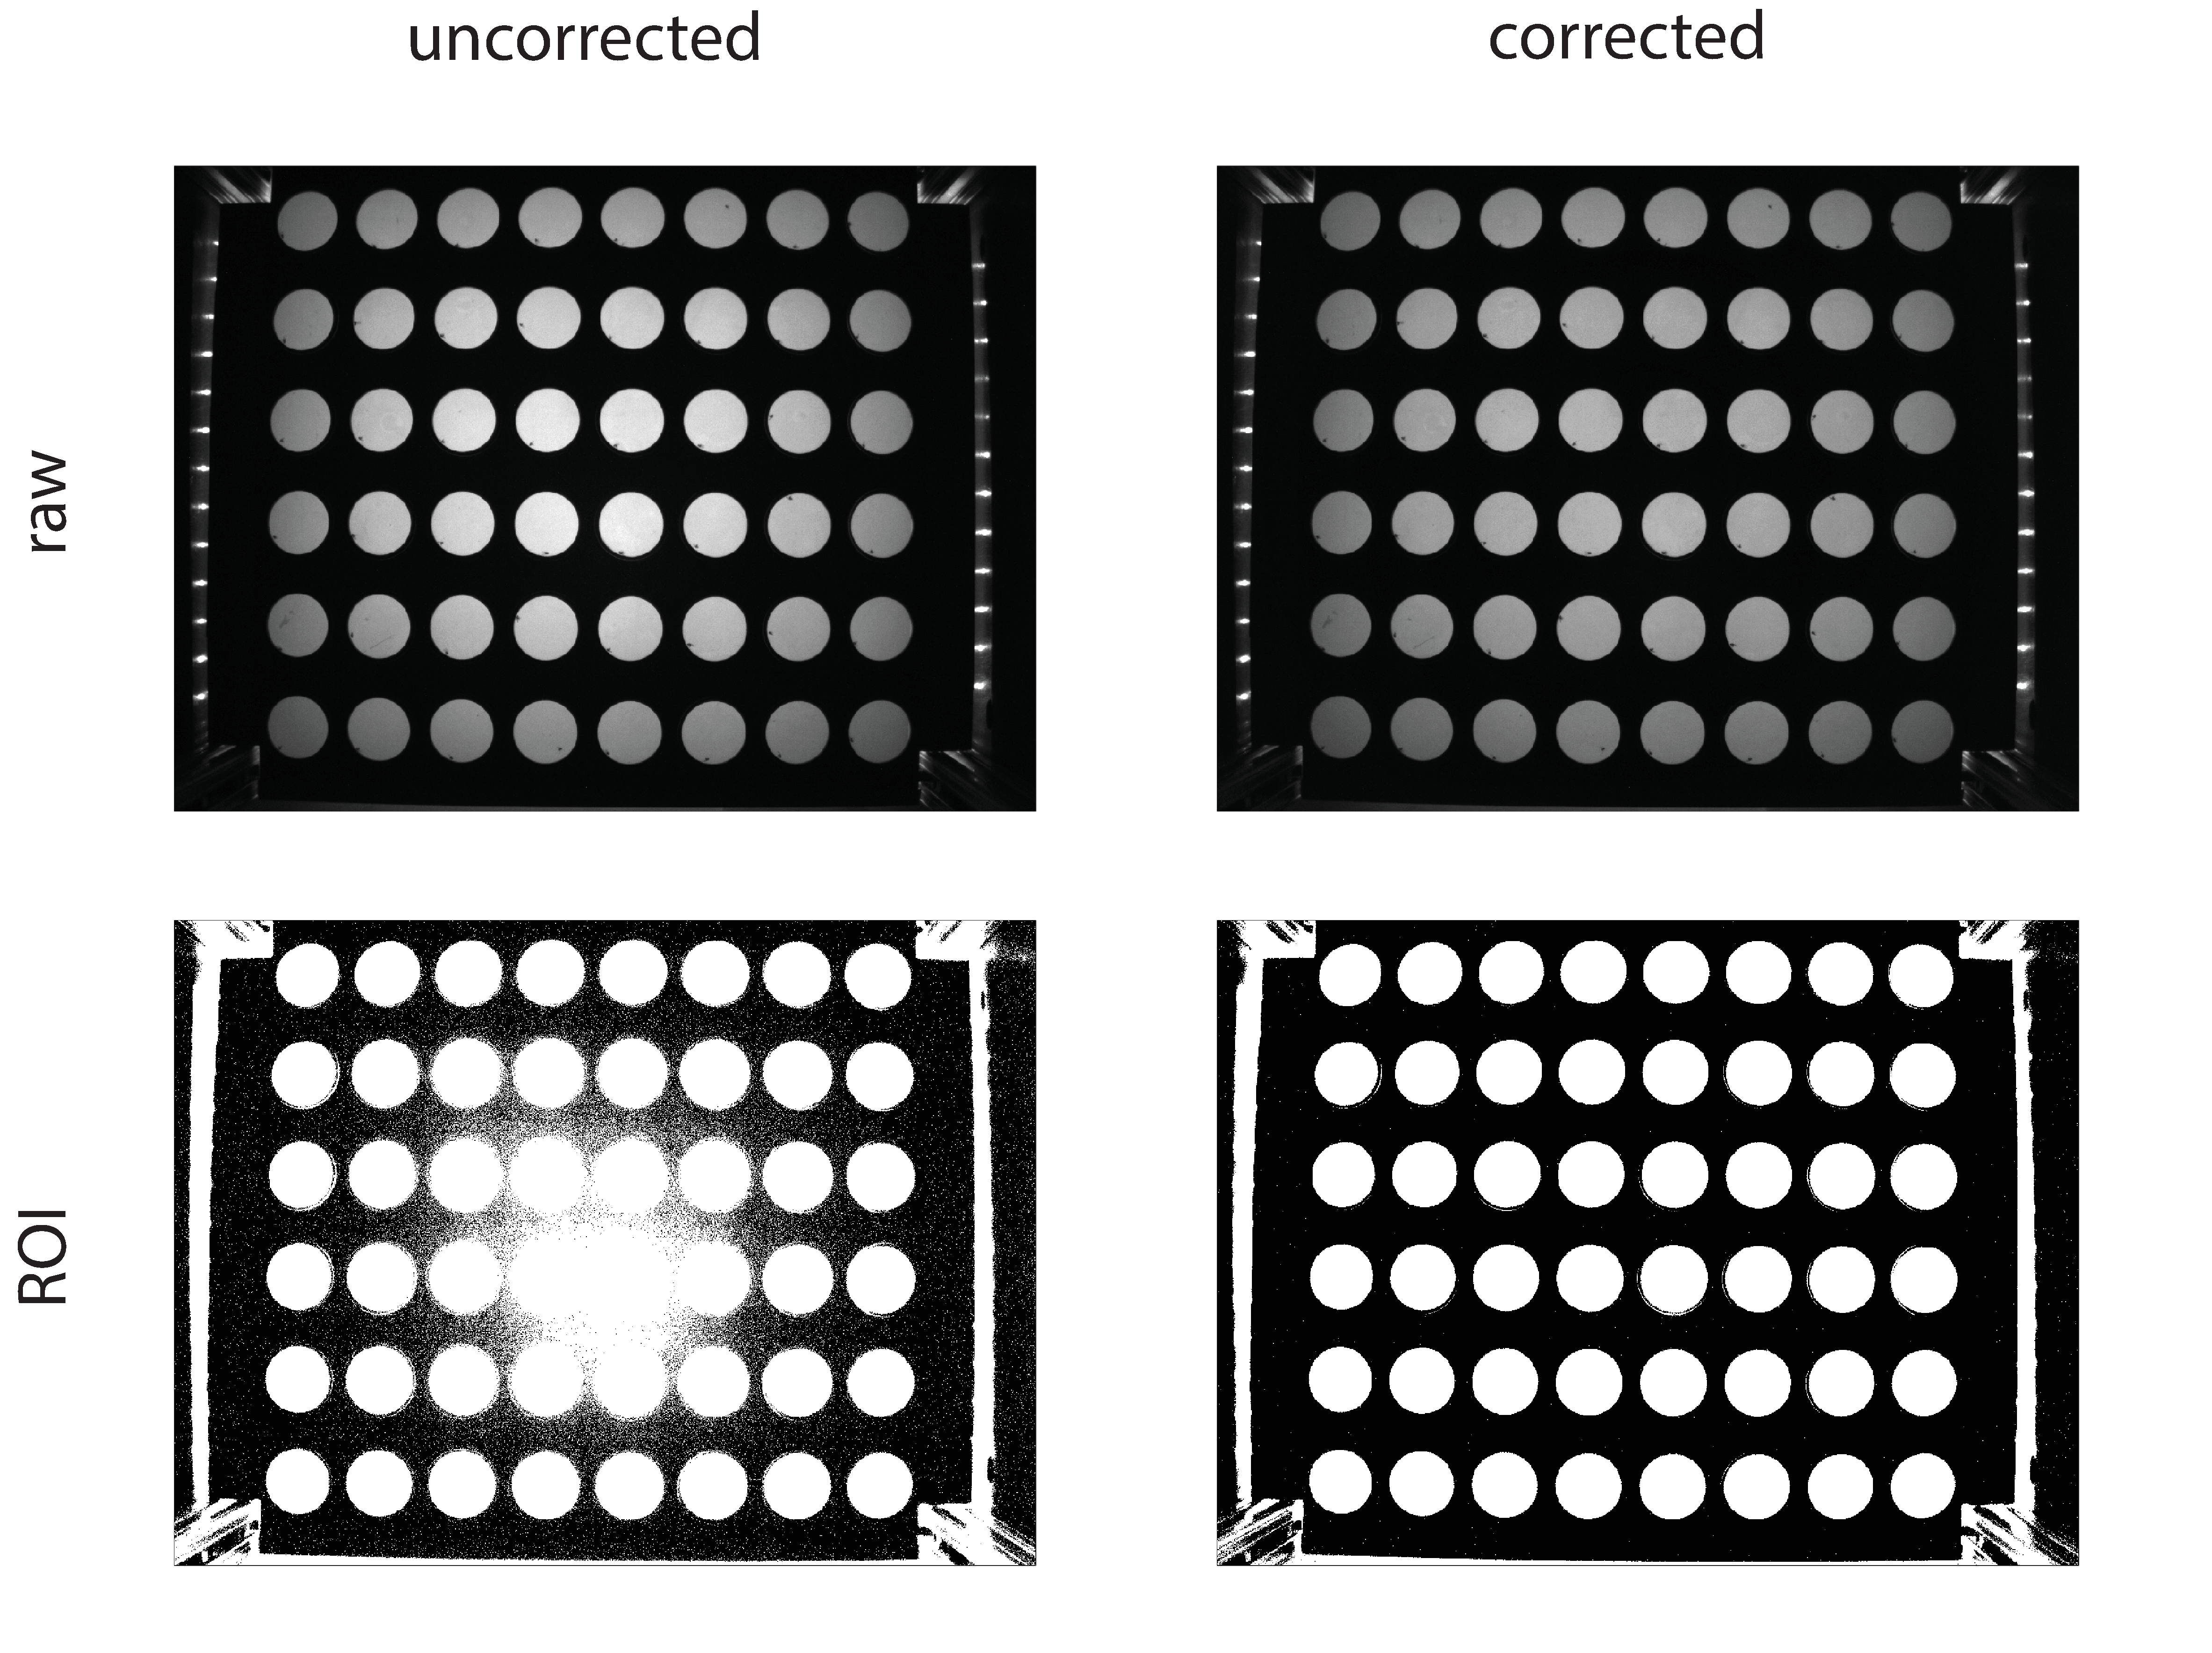
\includegraphics[width=0.5\textwidth]{images/vignette_correction/vignette_correction.pdf}
		\caption*{\footnotesize {\textit{figure 5.4} - vignette correction can improve automatic ROI detection}}
	\end{center}
\end{figure}

\item \textbf{ROI-based correction} can only be employed after ROI detection because it relies on using ROI definitions to pick out dim ROIs in the image. Using this information, MARGO generates a subtraction matrix from the reference image. This matrix reduces all bright areas of image to the brightness of the dim ROI. This has the advantage of not assuming any particular shape to the variation in luminance across the image and often results in more even illumination than gaussian correction. A sample dim ROI can be picked manually by selecting \textbf{\textit{Tracking} $>$ \textit{vignetting}}. Click and drag in the camera preview window to select a region of the image at the target brightness.

\end{itemize}

\subsection{Video recording}

Raw video data can be streamed to disk simultaneous with tracking. Uncompressed video files are useful for software packages that train behavioral classifiers on the raw pixel data such as the \href{http://jaaba.sourceforge.net/}{Janelia Automatic Animal Behavior Annotator (JAABA)}. Videos can additionally be used for manual annotation behaviors  or fed back into MARGO or other tracking programs for independent validation of traces.

Toggle video recording by selecting \textbf{\textit{Tracking} $>$ \textit{video} $>$ \textit{record}}. By default, MARGO saves uncompressed video data. Because raw video files can be very large, compression can be toggled by selecting \textit{Tracking} $>$ \textit{video} $>$ \textit{compress}. It is strongly recommended that uncompressed videos are saved for any application using the raw pixel data as compression will result in the loss of information.

\hypertarget{trackingperformance}{\subsection{Tracking performance}}

Low frame rates are often sufficient to capture behavior and can help reduce files sizes and data processing. But closed-loop stimulus delivery may demand acquisition rates that far exceed these rates. MARGO's real-time tracking excels at applications requiring tight closed-loop feedback. By optimizing your setup, MARGO can easily achieve acquisition rates greater than 60Hz. Each of the following can limit tracking performance:

\begin{itemize}
	\itemsep0em
	\item background pixel noise
	\item \textit{grid} ROI detection mode
	\item camera frame rate
	\item low target rate set under \textbf{\textit{Tracking} $>$ \textit{tracking parameters}}
	\item unoptimized minimum and maximum area thresholds
	\item display update mode (disabled by selecting \textbf{\textit{Display} $>$ \textit{none}})
	\item blob dilation/erosion (disabled by setting dilation size = 0)
\end{itemize} 

\newpage
\section{Creating a Custom Experiment}

Every tracking protocol (eg.\textit{Basic Tracking}, \textit{Circadian} or \textit{Y-maze}) follows the same simple workflow consisting of a run file and an analysis file. An example of a custom experiment is shown below by building off of the tracking script for the \textit{\textbf{Basic Tracking}} protocol. 

\subsection{Run file template}
Use the \textit{Basic Tracking} run file located in \textit{$<$MARGO\_directory$>$/experiments/Basic Tracking/run\_basictracking.m} as a template for creating a custom run file. Each run file will consist of initialization, tracking, and clean-up routines.

\begin{figure}[h!]
	\begin{center}
		\vspace*{0.75cm}
		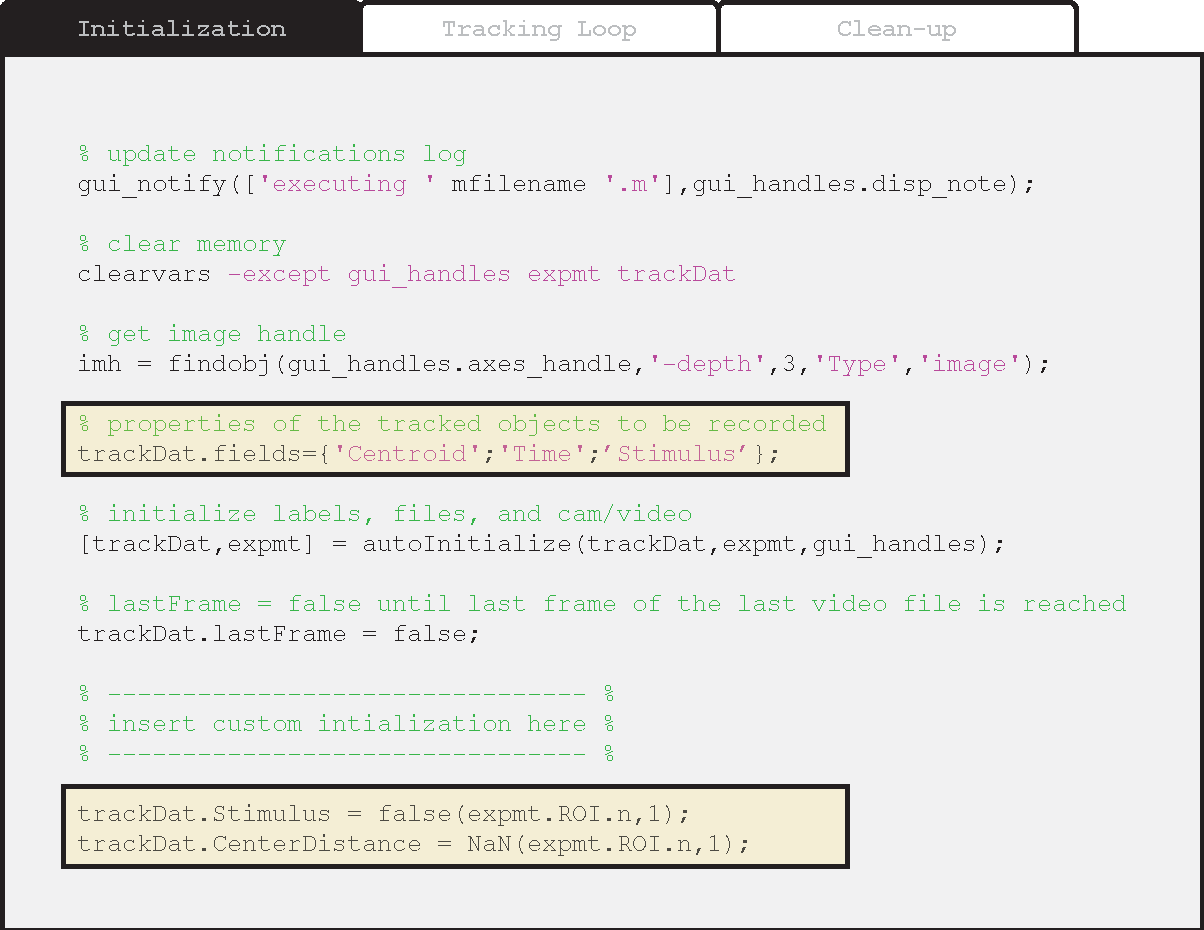
\includegraphics[width=1\textwidth]{images/custom_exp/initialization.pdf}
		\caption*{\footnotesize {\textit{figure 6.1.1} - The basic initialization template has been modified to include initialization of our custom fields (highlighted regions). The custom raw data field, \textit{Stimulus} has been added to the list of tracked fields so that the data will be written to the hard drive each frame. A second field has been initialized to store the distance of each object to the center of its ROI for the current frame.}}
	\end{center}
\end{figure}

\newpage
\textbf{\underline{Initialization}}\\
The initialization routine ensures that the camera, data files, and tracking variables are setup for tracking. The setup can simply be copied for most experiments with two notable exceptions:
\begin{itemize}
	\item Raw data fields are defined in \textbf{\textit{trackDat.fields}} and will automatically generate and save to raw data files in each frame. On each iteration of the tracking loop, the MARGO will to write any data in \textbf{\textit{trackDat.$<$field\_name$>$}} to the paired raw data file. This means that \textit{trackDat} must have an associated field for each entry to \textit{trackDat.fields}. For custom data fields, the field must be defined and updated in the tracking routine. The minimum tracked fields (ie. Centroid and Time) are defined in the example below (fig. 6.1.1). For this example, let's assume we want to trigger a stimulus delivery when tracked objects are close to the center of the ROI and that we want to save a raw data file that reads \textit{true} on frames where a stimulus was triggered and \textit{false} on any other frame. For this purpose, a custom data field \textit{Stimulus} has been added to the list of tracked fields. 
	\item Any custom parameters and values should be defined at the end of the initialization routine. This can be initialization of a custom data field described above or any temporary values that are not to be saved to a data file. Here we define our custom raw data field, \textit{trackDat.Stimulus}, and initialize it to \textit{false}. It has been defined as number of ROIs in length since each tracked individual will receive stimuli independently. It is worth noting that MARGO requires raw data fields to have the same dimensions and be of the same data type on each frame. We also define a field, \textit{trackDat.CenterDistance} that will not be saved since it is unlisted in \textit{trackDat.fields}.
\end{itemize}

\textbf{\underline{Tracking Loop}}\vspace*{0.25cm}\\
The main tracking loop consists of six core sub-routines essential to any experiment in MARGO:
\begin{enumerate}
	\itemsep0em
	\item update time-keeping variables
	\item query the next frame of data from camera or video file
	\item track objects in the current frame and match identities to previous frames
	\item write each field of raw data in \textit{trackDat.fields} to the hard drive
	\item check to see if the background reference needs to be updated
	\item update the display if necessary
\end{enumerate} 

Most custom experiments can be accomplished without altering any of the core sub-routines. In most cases, a single sub-routine between steps 3-4 to define in custom data fields and implement hardware control. Between steps 3-4, objects have already been tracked and have had their identities matched to traces from previous frames, but the data has not yet been written to the hard drive(fig. 6.1.2). This makes it simple to write a single function to filter existing fields or define custom fields for raw data saving. In this example, a function (\textit{customStimulusSubRoutine}) has been included to find tracked objects within some threshold distance to the center of its ROI (fig. 6.1.3). The result is stored in the raw data field \textit{trackDat.Stimulus} and is used to filter which ROIs receive a stimulus.  

\begin{figure}[h!]
	\begin{center}
		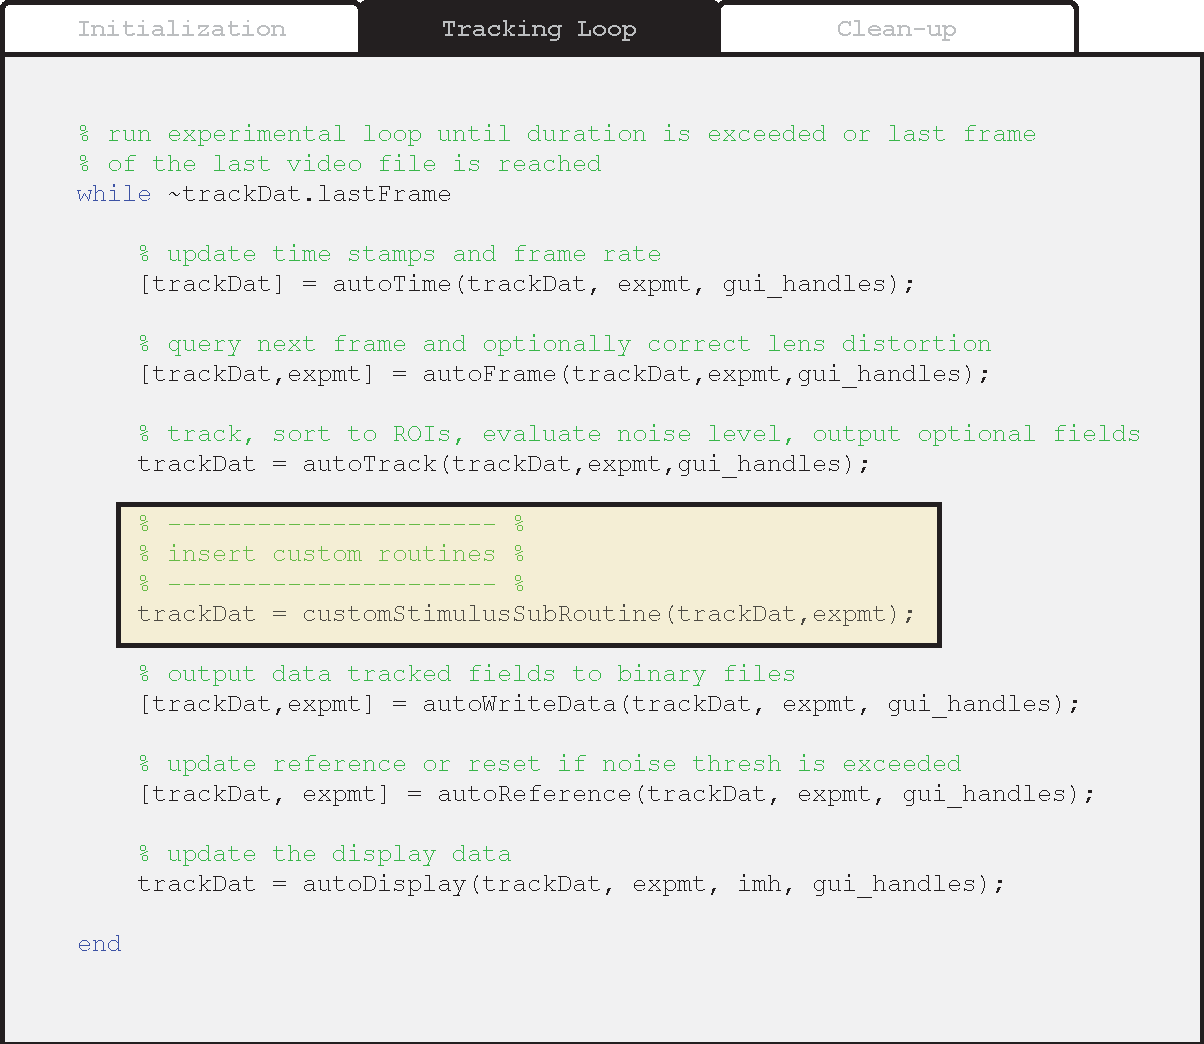
\includegraphics[width=0.8\textwidth]{images/custom_exp/tracking_loop.pdf}
		\caption*{\footnotesize {\textit{figure 6.1.2} - Custom routines (highlighted) can be called between steps 3-4 to define custom data fields and implement hardware control.}}
	\end{center}
\end{figure}

\begin{figure}[h!]
	\begin{center}
		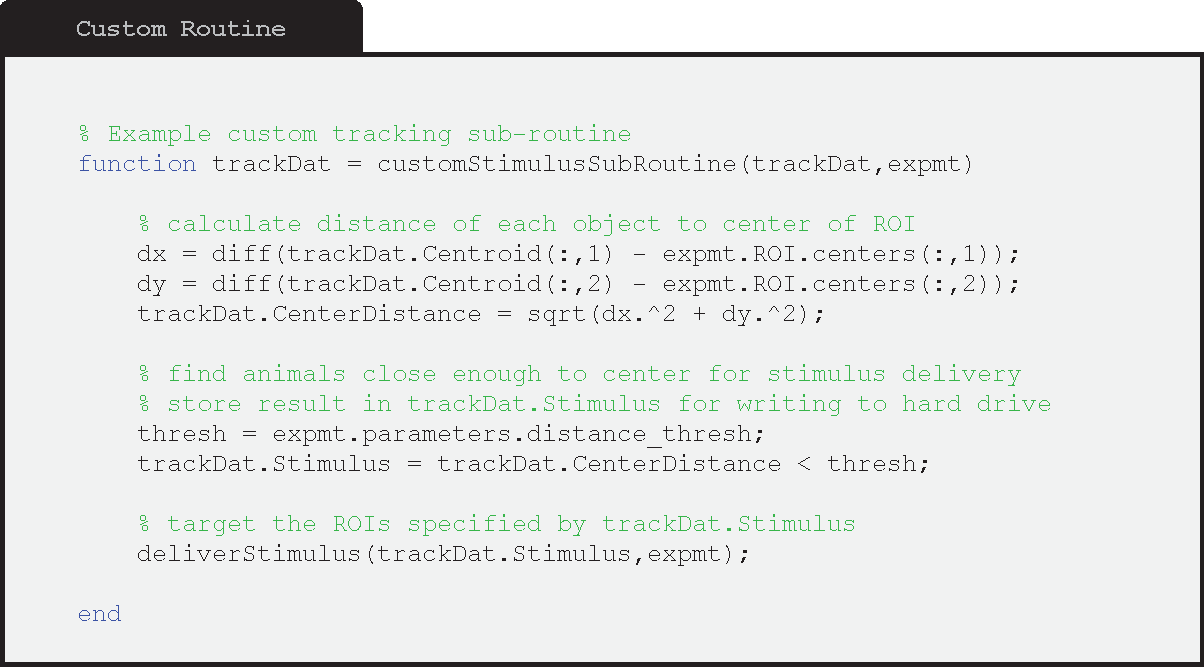
\includegraphics[width=0.8\textwidth]{images/custom_exp/custom_routine.pdf}
		\caption*{\footnotesize {\textit{figure 6.1.3} - Example custom routine where our raw data field is assigned prior to writing data to the hard drive. Distance to center is calculated and compared to a threshold value (defined outside of the run file our during initialization). The data is then passed to a hypothetical function that delivers stimuli to the ROIs specified by \textit{trackDat.Stimulus}.}}
	\end{center}
\end{figure}

\newpage
\textbf{\underline{Clean-up}}

The clean-up routine will be largely the same for all tracking experiments and consists primarily of the \textit{autoFinish} sub-routine. The \textit{autoFinish} sub-routine executes by default unless flagged by the user by selecting \textbf{\textit{Stop}} $>$ \textbf{\textit{Delete}}, which removes all data files and directories associated with the experiment. During clean-up, the \textit{ExperimentData} master data container is updated and re-saved before analysis, raw data files are closed, temporary display objects are removed, the camera is stopped, and outputs to the run file are assigned. Insert code for shutting down external hardware or cleaning up the UI here.

\begin{figure}[h!]
	\vspace*{0.75cm}
	\begin{center}
		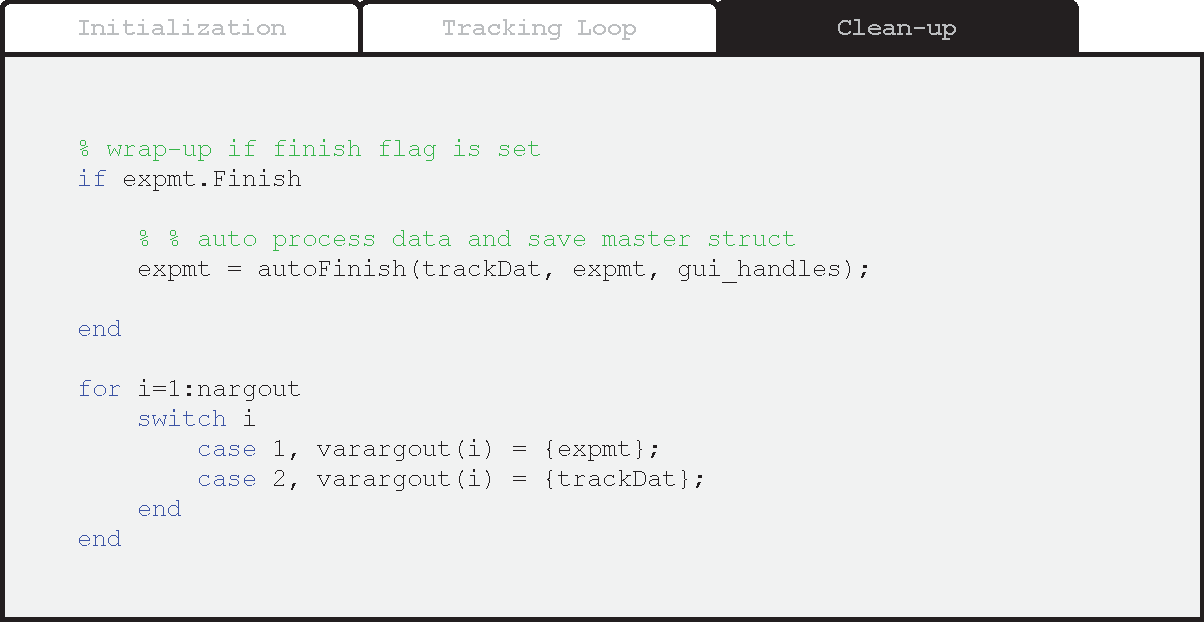
\includegraphics[width=0.8\textwidth]{images/custom_exp/clean_up.pdf}
		\caption*{\footnotesize {\textit{figure 6.1.4} - The finish sub-routine backups the \textit{\textit{ExperimentData}} .mat file, cleans the UI, shuts down open hardware sessions, and closes raw data files.}}
	\end{center}
\end{figure}

\newpage
\subsection{Analyze file template}

The analysis template consists of two core sub-routines useful for interfacing with MARGO data files: \textit{autoDataProcess} and \textit{autoFinishAnalysis}.

\textbf{\underline{autoDataProcess}}
\begin{itemize}
	\itemsep0em
	\item parses name-value pairs for data processing options
	\item initializes the processing \textit{options} struct
	\item initializes memmap objects for accessing the raw data files
	\item calculates and saves trace features (\textit{optional})
	\begin{itemize}
		\itemsep0em
		\item speed
		\item heading angle
		\item four quadrant inverse tangent
		\item distance to ROI center
	\end{itemize}
	\item parses traces into discreet movement bouts (\textit{optional})
	\item corrects speed data for fisheye lens distortion (\textit{optional})
\end{itemize}
\textbf{\underline{autoFinishAnalysis}}
\begin{itemize}
	\itemsep0em
	\item re-saves \textit{\textit{ExperimentData}} struct following analysis
	\item closes open raw data files
	\item resets the \textit{\textit{ExperimentData}} struct for next experiment
\end{itemize}

\begin{figure}[h!]
	\begin{center}
		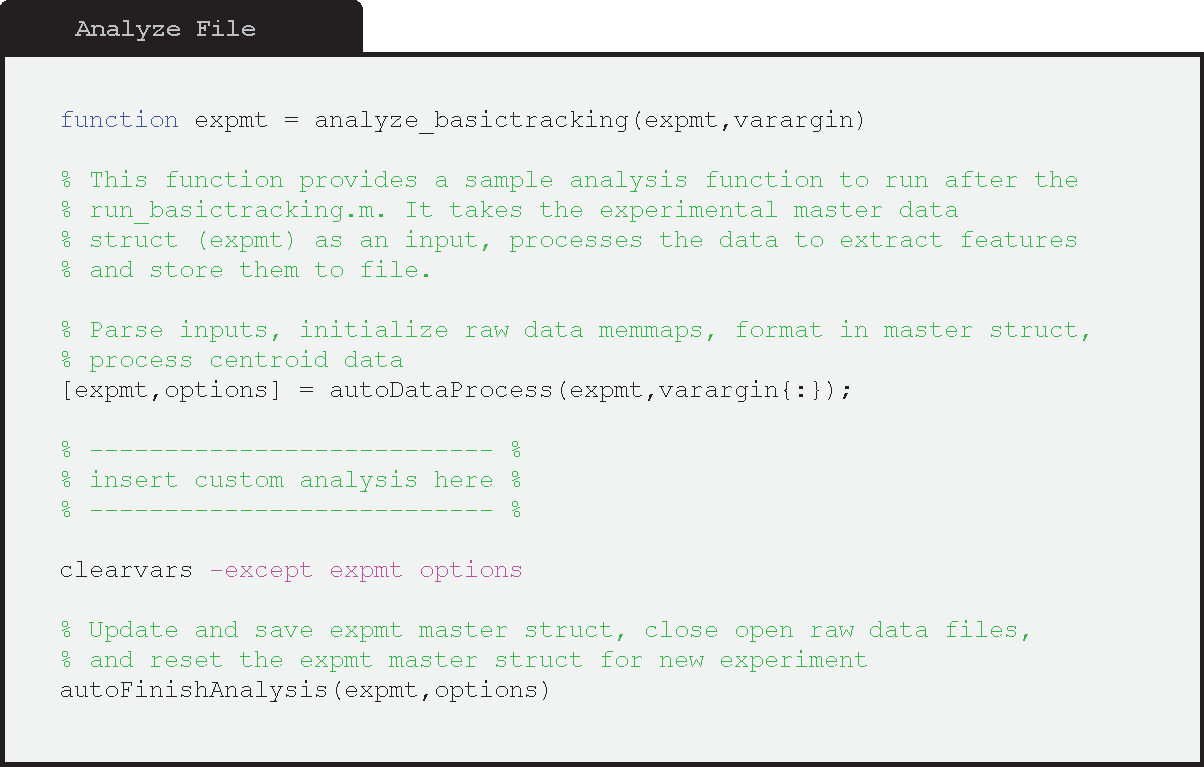
\includegraphics[width=0.8\textwidth]{images/custom_exp/analysis.pdf}
		\caption*{\footnotesize {\textit{figure 6.1.4} - The finish sub-routine backups the \textit{\textit{ExperimentData}} .mat file, cleans the UI, shuts down open hardware sessions, and closes raw data files.}}
	\end{center}
\end{figure}



\newpage
\section{Visual Stimulus Delivery with Psychtoolbox}

MARGO supports closed-loop targeting of visual stimuli to individual ROIs using an external display or projector. Visual stimuli can be crafted and displayed with \href{http://psychtoolbox.org/overview/}{Psychtoolbox}, a freely-available, MATLAB based software package for psychology and neuroscience research. Psychtoolbox is not included with MARGO and must be \href{http://psychtoolbox.org/download/}{downloaded and installed} separately. Psychtoolbox is an incredibly powerful and expansive package developed by Mario Kleiner. See one of the many \href{http://peterscarfe.com/ptbtutorials.html}{online resources} to learn how to generate and display stimuli.

\subsection{Projector box}

Mounting an overhead projector to the behavioral box allows targeting of visual stimuli to individual ROIs. The camera can be placed slightly off-center so the behavioral platform is visible to both the camera and projector. Equipping a long-pass filter to the camera allows tracking done in infrared without interference from the projector (fig. 8.1). 

\begin{figure}[h!]
	\begin{center}
		\includegraphics[width=0.95\textwidth]{images/projector/proj_schematic.pdf}
		\caption*{\footnotesize {\textit{figure 8.1} - Sample schematic of projector behavioral box. An external long-pass filter can be rotated in and out of the imaging path allowing the camera to switch between imaging only infrared light and imaging both infrared and visible light. The overhead projector targets individual ROIs underneath by projecting visual stimuli on a diffuser film on the floor of the behavioral arenas.}}
	\end{center}
\end{figure}

In order to accurately target objects within the camera's field of view with the projector, a mapping must be made between the pixel coordinates of both the camera and projector. MARGO creates this mapping by tracking a spot that is rastered through the projector's display. For this to work, the projection must be visible to the camera during registration but invisible to the camera during tracking. Mounting a long-pass filter on a swivel makes it easy to switch between the two without disturbing the camera.

\subsection{Registering the projector to the camera}

Any coordinate mapping between the camera and the projector will only accurate for a particular configuration and positioning of both. If either is moved during or after registration, the process must be started over again to have an accurate mapping. Having a high contrast, non-reflective projection surface will greatly improve the ease of tracking the projector with the camera. A flat white sheet of paper or matte white painted surface works well. Do the following to register the projector in MARGO:

\begin{enumerate}
	\item Ensure that Psychtoolbox is installed by executing \textbf{\textit{PsychtoolboxVersion}} in the MATLAB command window (MARGO support built on version 3)
	\item Remove the infrared filter from the imaging path and start the camera preview
	\item Place a high-contrast, white surface on the behavioral platform
	\item Ensure no sources of illumination but the projector will be visible to the camera 
	\item Drag a window into the projector display (anything with high-contrast black and white text) and ensure the projector is in focus
	\item Adjust the camera aperture or exposure (under camera settings) and focus until the projector display is clearly visible in the camera preview
	\item Select \textbf{\textit{Hardware}} $>$ \textbf{\textit{projector}} $>$ \textbf{\textit{register projector}}
	\item Select and confirm the projector screen and registration parameters when prompted to begin registration
		\begin{itemize}
			\item \textit{Grid Step Size} sets how finely the projector rasters its field of view
			\item \textit{Spot Radius} sets the size of the rastered dot (the apparent size should be between 1-5\% the area of the camera)
		\end{itemize}
	\item Once registration is finished, the output mapping will be saved to file under: \newline \textbf{\textit{\texttildelow MARGO/hardware/projector\_fit/}}
\end{enumerate}

\subsection{Using registration output in experiments}

Once registration is complete, no additional configuration of the projector or registration mapping is required to run the prepackaged \textit{\textbf{Optomotor}}, \textbf{\textit{Slow Phototaxis}}, and \textbf{\textit{Temporal Phototaxis}} experiments. To use the mapping in custom experiments, run the following command: 

\begin{center}
	\textit{\textit{ExperimentData} = initialize\_projector(\textit{ExperimentData}, bg\_color)}
\end{center}

This initializes a Psychtoolbox window to the screen set under registration parameters with the background color specified by the RGB triplet, \textit{bg\_color}. Additionally, projector initialization stores the registration mapping and screen properties to the \textit{\textit{ExperimentData}} struct. To convert from camera coordinates to projector coordinates, use the 2D scattered interpolants stored under \textit{\textit{ExperimentData}.projector}:

\begin{center}
	\textit{projector\_x = \textit{ExperimentData}.projector.Fx(cam\_x, cam\_y)};\\
	\textit{projector\_y = \textit{ExperimentData}.projector.Fy(cam\_x, cam\_y)};
\end{center}

\begin{figure}[h!]
	\begin{center}
		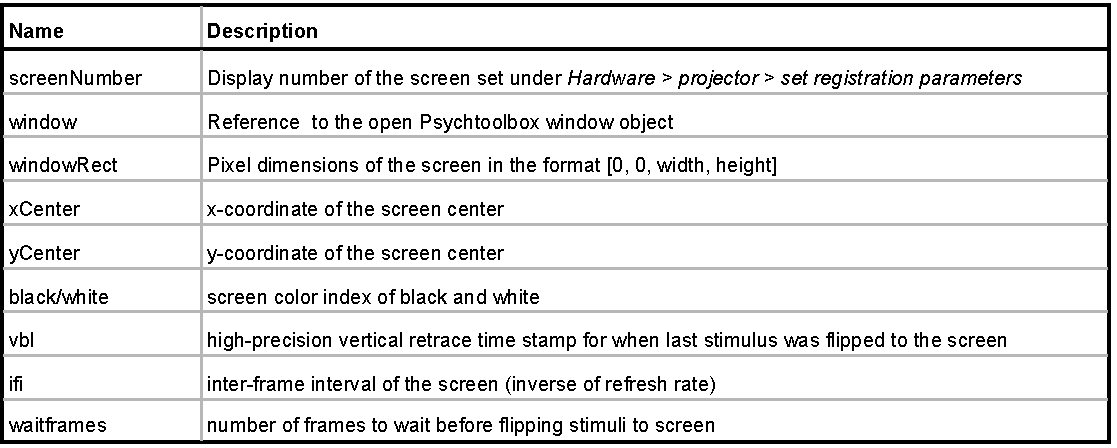
\includegraphics[width=0.95\textwidth]{images/projector/scrProps.pdf}
		\caption*{\footnotesize {\textit{Table 8.3} - Field names and descriptions of the screen properties output to \textit{\textit{ExperimentData}.scrProp} following projector initialization. The properties stored here be used to accurately time and display stimuli to the Pyschtoolbox window opened during initialization.}}
	\end{center}
\end{figure}

Detailed use of MARGO and Psychtoolbox to deliver stimuli under closed-loop control is beyond the scope of this manual, but sample implementations are available in \textbf{\textit{run\_optomotor.m}} and \textbf{\textit{run\_slowphototaxis.m}}.




\newpage
\section{Tracking with Video Input}

MARGO accepts video files as an input source for tracking. Select \textit{Source} $>$ \textit{video file} to switch inputs. Many programs will output raw video data in \textit{avi2} format, which has a 2GB file size limit. When the file size limit is reached, subsequent files are automatically generated. To allow sequential tracking across multiple files, MARGO will automatically track all videos under the target directory. The software makes the assumption that all files under the same directory belong to the same experiment and will only generate a single .mat output file. The software can take \textit{.avi}, \textit{.mp4}, \textit{.m4v}, \textit{.mov}, \textit{.wmv} and \textit{.mpg} file formats as input. Because video files are not tracked in real time, the time-stamps output from video file tracking are inferred from the frame rate of the file and may not be accurate.


\end{document}